% Autor: Chris Lippe, Jonathan Sigrist, Jannik Tim Zarnitz
% Datum: 2019-11
% basiert auf der Vorlage für Versuchsprotokolle von Simon May

\documentclass[
a4paper,                % Papierformat (DIN A4)
titlepage=firstiscover, % Separate Titelseite
captions=tableheading,  % \caption bei Tabellen immer als Überschrift setzen
toc=bibliography,       % Literaturverzeichnis im Inhaltsverzeichnis aufführen
toc=listof,             % Abbildungsverzeichnis etc. im Inhaltsverzeichnis aufführen
oneside,                % Einseitig
%twoside,               % Zweiseitig
%twocolumn,             % Zweispaltig
automark,               % Abschnittstitel automatisch in Kopfzeile einfügen
12pt,                   % Schriftgröße (beliebige Größen mit „fontsize=Xpt“)
english, ngerman,       % Sprache für z.B. Babel; ausgewählt: ngerman (letztgenannt)
%draft=true             % Entwurf-Modus; markiert zu lange und zu kurze Zeilen
parskip = half,         % Abstand nach Absatz
]{scrartcl}

% Autor: Simon May
% Datum: 2017-10-04

% --- Pakete einbinden
% --- Pakete erweitern LaTeX um zusätzliche Funktionen.
%     Dies ist ein Satz nützlicher Pakete.

% Silbentrennung etc.; Sprache wird durch Option bei \documentclass festgelegt
\usepackage{babel}
\usepackage{iftex}
\ifLuaTeX
	% Schriftart (Latin Modern)
	\usepackage{fontspec}
	\fontspec{Latin Modern Roman}
\else
	% Verwendung der Zeichentabelle T1 (für Sonderzeichen etc.)
	\usepackage[T1]{fontenc}
	% Legt die Eingabe-Zeichenkodierung fest, z.B. UTF-8
	\usepackage[utf8]{inputenc}
	% Schriftart (Latin Modern)
	\usepackage{lmodern}
	% Zusätzliche Sonderzeichen
	\usepackage{textcomp}
\fi

\usepackage{upgreek}

% Nutzen von +, -, *, / in \setlength u.ä. (z.B. \setlength{\a + 3cm})
\usepackage{calc}
% Wird benötigt, um \ifthenelse zu benutzen
\usepackage{xifthen}
% Optionen für eigene definierte Befehle
\usepackage{xparse}

% Verbessertes Aussehen des Schriftbilds durch kleine Anpassungen
\usepackage{microtype}
% Automatische Formatierung von Daten
\usepackage[useregional]{datetime2}
% Wird für Kopf- und Fußzeile benötigt
\usepackage{scrlayer-scrpage}
% Einfaches Wechseln zwischen unterschiedlichen Zeilenabständen
\usepackage{setspace}
% Optionen für Listen (enumerate, itemize, …)
\usepackage{enumitem}
% Automatische Anführungszeichen
\usepackage{csquotes}
% Zusätzliche Optionen für Tabellen (tabular)
\usepackage{array}

% Mathepaket (intlimits: Grenzen über/unter Integralzeichen)
\usepackage[intlimits]{amsmath}
% Mathe-Symbole, \mathbb etc.
\usepackage{amssymb}
% Weitere Mathebefehle
\usepackage{mathtools}
% „Schöne“ Brüche im Fließtext
\usepackage{xfrac}
% Ermöglicht die Nutzung von \SI{Zahl}{Einheit} u.a.
\usepackage{siunitx}
% Ermöglicht Nutzung von \pdv als Ableitungen
\usepackage{physics}
% Definition von Unicode-Symbolen; Nach [utf8]inputenc laden!
\usepackage{newunicodechar}
% Unicode-Formeln mit pdfLaTeX
% Autor: Simon May
% Datum: 2015-03-04

% Diese Datei ermöglicht es, Mathe-Symbole (z.B. \gamma) direkt als
% Sonderzeichen (d.h. γ) einzugeben

% silence unterdrückt Warnungen; vor hyperref laden
\usepackage{silence}
\WarningFilter[pdflatex-unicode-math]{newunicodechar}{Redefining Unicode character}
\ActivateWarningFilters[pdflatex-unicode-math]

\newunicodechar{†}{\dag}
\newunicodechar{‡}{\ddag}
\newunicodechar{…}{\ldots}
\newunicodechar{⋯}{\cdots}
\newunicodechar{⋮}{\vdots}
\newunicodechar{⋱}{\ddots}
\newunicodechar{⋰}{\iddots}
\newunicodechar{α}{\alpha}
\newunicodechar{β}{\beta}
\newunicodechar{γ}{\gamma}
\newunicodechar{δ}{\delta}
\newunicodechar{ε}{\varepsilon}
\newunicodechar{ϵ}{\epsilon}
\newunicodechar{ζ}{\zeta}
\newunicodechar{η}{\eta}
\newunicodechar{θ}{\theta}
\newunicodechar{ϑ}{\vartheta}
\newunicodechar{ι}{\iota}
\newunicodechar{κ}{\kappa}
\newunicodechar{ϰ}{\varkappa}
\newunicodechar{λ}{\lambda}
\newunicodechar{μ}{\mu}
\newunicodechar{ν}{\nu}
\newunicodechar{ξ}{\xi}
\newunicodechar{ο}{o}
\newunicodechar{π}{\pi}
\newunicodechar{ρ}{\rho}
\newunicodechar{ϱ}{\varrho}
\newunicodechar{σ}{\sigma}
\newunicodechar{τ}{\tau}
\newunicodechar{υ}{\upsilon}
\newunicodechar{φ}{\varphi}
\newunicodechar{ϕ}{\phi}
\newunicodechar{χ}{\chi}
\newunicodechar{ψ}{\psi}
\newunicodechar{ω}{\omega}
\newunicodechar{Α}{\mathrm{A}}
\newunicodechar{Β}{\mathrm{B}}
\newunicodechar{Γ}{\Gamma}
\newunicodechar{Δ}{\Delta}
\newunicodechar{Ε}{\mathrm{E}}
\newunicodechar{Ζ}{\mathrm{Z}}
\newunicodechar{Η}{\mathrm{H}}
\newunicodechar{Θ}{\Theta}
\newunicodechar{Ι}{\mathrm{I}}
\newunicodechar{Κ}{\mathrm{K}}
\newunicodechar{Λ}{\Lambda}
\newunicodechar{Μ}{\mathrm{M}}
\newunicodechar{Ν}{\mathrm{N}}
\newunicodechar{Ξ}{\Xi}
\newunicodechar{Ο}{\mathrm{O}}
\newunicodechar{Π}{\Pi}
\newunicodechar{Ρ}{\mathrm{P}}
\newunicodechar{Σ}{\Sigma}
\newunicodechar{Τ}{\mathrm{T}}
\newunicodechar{Υ}{\Upsilon}
\newunicodechar{Φ}{\Phi}
\newunicodechar{Χ}{\Chi}
\newunicodechar{Ψ}{\Psi}
\newunicodechar{Ω}{\Omega}
\newunicodechar{∑}{\sum}
\newunicodechar{∫}{\int}
\newunicodechar{∬}{\iint}
\newunicodechar{∭}{\iiint}
\newunicodechar{⨌}{\iiiint}
\newunicodechar{∮}{\oint}
\newunicodechar{∯}{\oiint}
\newunicodechar{∰}{\oiiint}
\newunicodechar{∇}{\nabla}
\newunicodechar{∂}{\partial}
\newunicodechar{√}{\sqrt}
\newunicodechar{∈}{\in}
\newunicodechar{∋}{\ni}
\newunicodechar{∉}{\notin}
\newunicodechar{∀}{\forall}
\newunicodechar{∃}{\exists}
\newunicodechar{∄}{\nexists}
\newunicodechar{∴}{\therefore}
\newunicodechar{∵}{\because}
\newunicodechar{〈}{\langle}
\newunicodechar{〉}{\rangle}
\newunicodechar{⌊}{\lfloor}
\newunicodechar{⌋}{\rfloor}
\newunicodechar{⌈}{\lceil}
\newunicodechar{⌉}{\rceil}
\newunicodechar{∼}{\sim}
\newunicodechar{∝}{\propto}
\newunicodechar{∞}{\infty}
\newunicodechar{ℵ}{\aleph}
\newunicodechar{ℏ}{\hbar}
\newunicodechar{℘}{\wp}
\newunicodechar{ℓ}{\ell}
\newunicodechar{∅}{\emptyset}
\newunicodechar{×}{\times}
\newunicodechar{⋅}{\cdot}
\newunicodechar{÷}{\div}
\newunicodechar{⋆}{\star}
\newunicodechar{∘}{\circ}
\newunicodechar{⋄}{\diamond}
\newunicodechar{⊕}{\oplus}
\newunicodechar{⊖}{\ominus}
\newunicodechar{⊗}{\otimes}
\newunicodechar{⊘}{\oslash}
\newunicodechar{⊙}{\odot}
\newunicodechar{±}{\pm}
\newunicodechar{∓}{\mp}
\newunicodechar{≈}{\approx}
\newunicodechar{≡}{\equiv}
\newunicodechar{≠}{\ne}
\newunicodechar{≥}{\ge}
\newunicodechar{≤}{\le}
\newunicodechar{≫}{\gg}
\newunicodechar{≪}{\ll}
\newunicodechar{⊂}{\subset}
\newunicodechar{⊃}{\supset}
\newunicodechar{⊆}{\subseteq}
\newunicodechar{⊇}{\supseteq}
\newunicodechar{⊈}{\nsubseteq}
\newunicodechar{⊉}{\nsupseteq}
\newunicodechar{≔}{\coloneqq}
\newunicodechar{≕}{\eqqcolon}
\newunicodechar{¬}{\neg}
\newunicodechar{∨}{\vee}
\newunicodechar{∧}{\wedge}
\newunicodechar{∪}{\cup}
\newunicodechar{∩}{\cap}
\newunicodechar{⋁}{\bigvee}
\newunicodechar{⋀}{\bigwedge}
\newunicodechar{⋃}{\bigcup}
\newunicodechar{⋂}{\bigcap}
\newunicodechar{⟂}{\perp}
\newunicodechar{∥}{\parallel}
\newunicodechar{∦}{\nparallel}
\newunicodechar{𝚤}{\imath}
\newunicodechar{𝚥}{\jmath}
\newunicodechar{⇔}{\Leftrightarrow}
\newunicodechar{⇕}{\Updownarrow}
\newunicodechar{⇐}{\Leftarrow}
\newunicodechar{⇒}{\Rightarrow}
\newunicodechar{⇑}{\Uparrow}
\newunicodechar{⇓}{\Downarrow}
\newunicodechar{↔}{\leftrightarrow}
\newunicodechar{↕}{\updownarrow}
\newunicodechar{←}{\leftarrow}
\newunicodechar{→}{\rightarrow}
\newunicodechar{↑}{\uparrow}
\newunicodechar{↓}{\downarrow}
\newunicodechar{⟷}{\longleftrightarrow}
\newunicodechar{⟵}{\longleftarrow}
\newunicodechar{⟶}{\longrightarrow}
\newunicodechar{⇇}{\leftleftarrows}
\newunicodechar{⇉}{\rightrightarrows}
\newunicodechar{⇈}{\upuparrows}
\newunicodechar{⇊}{\downdownarrows}
\newunicodechar{⟺}{\Longleftrightarrow}
\newunicodechar{⟸}{\Longleftarrow}
\newunicodechar{⟹}{\Longrightarrow}
\newunicodechar{↦}{\mapsto}
\newunicodechar{↤}{\mapsfrom}
\newunicodechar{⟼}{\longmapsto}
\newunicodechar{⟻}{\longmapsfrom}
\newunicodechar{⟾}{\Longmapsto}
\newunicodechar{⟽}{\Longmapsfrom}
\newunicodechar{↗}{\nearrow}
\newunicodechar{↖}{\nwarrow}
\newunicodechar{↘}{\searrow}
\newunicodechar{↙}{\swarrow}
\newunicodechar{↩}{\hookleftarrow}
\newunicodechar{↪}{\hookrightarrow}
\newunicodechar{↶}{\curvearrowleft}
\newunicodechar{↷}{\curvearrowright}
\newunicodechar{↺}{\circlearrowleft}
\newunicodechar{↻}{\circlearrowright}
\newunicodechar{↫}{\looparrowleft}
\newunicodechar{↬}{\looparrowright}
\newunicodechar{⇋}{\leftrightharpoons}
\newunicodechar{⇌}{\rightleftharpoons}
\newunicodechar{↼}{\leftharpoonup}
\newunicodechar{↽}{\leftharpoondown}
\newunicodechar{⇀}{\rightharpoonup}
\newunicodechar{⇁}{\rightharpoondown}
\newunicodechar{↿}{\upharpoonleft}
\newunicodechar{↾}{\upharpoonright}
\newunicodechar{⇃}{\downharpoonleft}
\newunicodechar{⇂}{\downharpoonright}
\newunicodechar{𝔸}{\mathbb{A}}
\newunicodechar{𝔹}{\mathbb{B}}
\newunicodechar{ℂ}{\mathbb{C}}
\newunicodechar{𝔻}{\mathbb{D}}
\newunicodechar{𝔼}{\mathbb{E}}
\newunicodechar{𝔽}{\mathbb{F}}
\newunicodechar{𝔾}{\mathbb{G}}
\newunicodechar{ℍ}{\mathbb{H}}
\newunicodechar{𝕀}{\mathbb{I}}
\newunicodechar{𝕁}{\mathbb{J}}
\newunicodechar{𝕂}{\mathbb{K}}
\newunicodechar{𝕃}{\mathbb{L}}
\newunicodechar{𝕄}{\mathbb{M}}
\newunicodechar{ℕ}{\mathbb{N}}
\newunicodechar{𝕆}{\mathbb{O}}
\newunicodechar{ℙ}{\mathbb{P}}
\newunicodechar{ℚ}{\mathbb{Q}}
\newunicodechar{ℝ}{\mathbb{R}}
\newunicodechar{𝕊}{\mathbb{S}}
\newunicodechar{𝕋}{\mathbb{T}}
\newunicodechar{𝕌}{\mathbb{U}}
\newunicodechar{𝕍}{\mathbb{V}}
\newunicodechar{𝕎}{\mathbb{W}}
\newunicodechar{𝕏}{\mathbb{X}}
\newunicodechar{𝕐}{\mathbb{Y}}
\newunicodechar{ℤ}{\mathbb{Z}}
\newunicodechar{𝒜}{\mathcal{A}}
\newunicodechar{ℬ}{\mathcal{B}}
\newunicodechar{𝒞}{\mathcal{C}}
\newunicodechar{𝒟}{\mathcal{D}}
\newunicodechar{ℰ}{\mathcal{E}}
\newunicodechar{ℱ}{\mathcal{F}}
\newunicodechar{𝒢}{\mathcal{G}}
\newunicodechar{ℋ}{\mathcal{H}}
\newunicodechar{ℐ}{\mathcal{I}}
\newunicodechar{𝒥}{\mathcal{J}}
\newunicodechar{𝒦}{\mathcal{K}}
\newunicodechar{ℒ}{\mathcal{L}}
\newunicodechar{ℳ}{\mathcal{M}}
\newunicodechar{𝒩}{\mathcal{N}}
\newunicodechar{𝒪}{\mathcal{O}}
\newunicodechar{𝒫}{\mathcal{P}}
\newunicodechar{𝒬}{\mathcal{Q}}
\newunicodechar{ℛ}{\mathcal{R}}
\newunicodechar{𝒮}{\mathcal{S}}
\newunicodechar{𝒯}{\mathcal{T}}
\newunicodechar{𝒰}{\mathcal{U}}
\newunicodechar{𝒱}{\mathcal{V}}
\newunicodechar{𝒲}{\mathcal{W}}
\newunicodechar{𝒳}{\mathcal{X}}
\newunicodechar{𝒴}{\mathcal{Y}}
\newunicodechar{𝒵}{\mathcal{Z}}
\newunicodechar{𝕬}{\mathfrak{A}}
\newunicodechar{𝕭}{\mathfrak{B}}
\newunicodechar{𝕮}{\mathfrak{C}}
\newunicodechar{𝕯}{\mathfrak{D}}
\newunicodechar{𝕰}{\mathfrak{E}}
\newunicodechar{𝕱}{\mathfrak{F}}
\newunicodechar{𝕲}{\mathfrak{G}}
\newunicodechar{𝕳}{\mathfrak{H}}
\newunicodechar{𝕴}{\mathfrak{I}}
\newunicodechar{𝕵}{\mathfrak{J}}
\newunicodechar{𝕶}{\mathfrak{K}}
\newunicodechar{𝕷}{\mathfrak{L}}
\newunicodechar{𝕸}{\mathfrak{M}}
\newunicodechar{𝕹}{\mathfrak{N}}
\newunicodechar{𝕺}{\mathfrak{O}}
\newunicodechar{𝕻}{\mathfrak{P}}
\newunicodechar{𝕼}{\mathfrak{Q}}
\newunicodechar{𝕽}{\mathfrak{R}}
\newunicodechar{𝕾}{\mathfrak{S}}
\newunicodechar{𝕿}{\mathfrak{T}}
\newunicodechar{𝖀}{\mathfrak{U}}
\newunicodechar{𝖁}{\mathfrak{V}}
\newunicodechar{𝖂}{\mathfrak{W}}
\newunicodechar{𝖃}{\mathfrak{X}}
\newunicodechar{𝖄}{\mathfrak{Y}}
\newunicodechar{𝖅}{\mathfrak{Z}}

\DeactivateWarningFilters[pdflatex-unicode-math]


% Farben
\usepackage{xcolor}
% Einbinden von Grafiken (\includegraphics)
\usepackage{graphicx}
% .tex-Dateien mit \includegraphics einbinden
\usepackage{gincltex}
% Größere Freiheiten bei Dateinamen mit \includegraphics
\usepackage{grffile}
% Abbildungen im Fließtext
\usepackage{wrapfig}
% Zitieren, Bibliographie (Biber als Bibliographie-Programm verwenden!)
\usepackage[backend=biber]{biblatex}
% Abbildungen nebeneinander (subfigure, subtable)
\usepackage{subcaption}
\usepackage{float}

% Verlinkt Textstellen im PDF-Dokument (sollte am Ende geladen werden)
\usepackage[unicode]{hyperref}
% „Schlaue“ Referenzen (nach hyperref laden!)
\usepackage{cleveref}
%PDF einbinden
%\usepackage{pdfpages}
%Graphiken zeichnen
%\usepackage{tikz}
%\usetikzlibrary{angles,quotes,babel,3d}

% Autor: Simon May
% Datum: 2017-10-05

% Eigene Befehle eignen sich gut, um Abkürzungen für lange Befehle zu erstellen.
% So vermeidet man, dass man immer wieder dasselbe Konstrukt kopieren und
% einfügen muss und, wenn man dann doch etwas ändern will, an zahllosen Stellen
% im Dokument dieselbe Änderung vornehmen muss.
% Die Syntax ist die folgende:
% \newcommand{neuer Befahl}[Anzahl Parameter (optional)]{Inhalt}
% Das folgende Beispiel fügt ein Bild mit bestimmten vorgegebenen Optionen ein:
\newcommand{\centeredImage}[1]{
	\begin{figure}
		\centering
		\includegraphics[width=0.5\textwidth]{#1}
	\end{figure}
}
% #1 ist dabei ein Parameter, den man \centeredImage übergeben muss, also:
% \centeredImage{...}
% Benötigt man keine Parameter, dann lässt man [1] weg. Werden zusätzliche
% Parameter benötigt, dann kann man die Zahl auf maximal 9 erhöhen.

% Ein Befehl, um eine E-Mail-Adresse darzustellen bzw. automatisch zu verlinken
\newcommand{\email}[1]{\href{mailto:#1}{\texttt{#1}}}

% \arsinh etc.
\newcommand*{\arsinh}{\operatorname{arsinh}}
\newcommand*{\arcosh}{\operatorname{arcosh}}
\newcommand*{\artanh}{\operatorname{artanh}}
\newcommand*{\const}{\text{const.}}
\newcommand*{\ie}{i.\,e.\ }
\newcommand*{\zB}{z.\,B.\ }
% Autor: Simon May
% Datum: 2016-10-13
% Der Befehl \newcommand kann auch benutzt werden, um „Variablen“ zu definieren:

% Nummer laut Praktikumsheft:
\newcommand*{\varNum}{V7}
% Name laut Praktikumsheft:
\newcommand*{\varName}{$\gamma$-$\gamma$-Winkelkorrelation}
% Datum der Durchführung:
\newcommand*{\varDatum}{25.11.2019}
% Autoren des Protokolls:
\newcommand*{\varAutor}{C. Lippe, J. Sigrist, J. T. Zarnitz}
\newcommand*{\varNameA}{Chris Lippe}
\newcommand*{\varNameB}{Jonathan Sigrist}
\newcommand*{\varNameC}{Jannik Tim Zarnitz}
% Nummer der eigenen Gruppe:
\newcommand*{\varGruppe}{Gruppe Ma-A-06}
% E-Mail-Adressen der Autoren:
\newcommand{\varEmailA}{c\_lipp02@wwu.de}
\newcommand{\varEmailB}{j\_sigrist@wwu.de}
\newcommand{\varEmailC}{j\_zarn02@wwu.de}
%betreuer Name
\newcommand{\varBetreuer}{Benjamin Hetz}
% E-Mail-Adresse anzeigen (true/false):
\newcommand*{\varZeigeEmail}{true}
% Kopfzeile anzeigen (true/false):
\newcommand*{\varZeigeKopfzeile}{true}
% Inhaltsverzeichnis anzeigen (true/false):
\newcommand*{\varZeigeInhaltsverzeichnis}{true}
% Literaturverzeichnis anzeigen (true/false):
\newcommand*{\varZeigeLiteraturverzeichnis}{true}

\newboolean{showEmail}
\setboolean{showEmail}{\varZeigeEmail}
\newboolean{showHeader}
\setboolean{showHeader}{\varZeigeKopfzeile}
\newboolean{showTOC}
\setboolean{showTOC}{\varZeigeInhaltsverzeichnis}
\newboolean{showBibliography}
\setboolean{showBibliography}{\varZeigeLiteraturverzeichnis}


% --- Einstellungen
% -- LaTeX/KOMA
% 1,5-facher Zeilenabstand
\onehalfspacing
\recalctypearea
% Schrift bei Bildunterschriften ändern
\addtokomafont{caption}{\small}
\addtokomafont{captionlabel}{\bfseries}
% Nummerierung der Formeln entsprechend des Abschnitts (z.B. 1.1)
\numberwithin{equation}{section}
% „Verwaiste“ Zeilen am Seitenanfang/-Ende stärker vermeiden
\clubpenalty=1000
\widowpenalty=1000
% Auf mehrere Seiten aufgespaltene Fußnoten stärker vermeiden
\interfootnotelinepenalty=3000

% -- csquotes
% Anführungszeichen automatisch umwandeln
\MakeOuterQuote{"}

% -- siunitx
\sisetup{
	locale=DE,
	separate-uncertainty,
	output-product=\cdot,
	quotient-mode=fraction,
	per-mode=fraction,
	fraction-function=\sfrac
	%inter-unit-product =${}\cdot{}$
	%number-unit-product = \,
}

% -- hyperref
\hypersetup{
	% Links/Verweise mit Kasten der Dicke 0.5pt versehen
	pdfborder={0 0 0.5}
	pdftitle={Versuchsprotokoll: \varName},
	pdfauthor={\varAutor},
	pdfsubject={Masterpraktikum},
	pdfkeywords={Physik, Münster, Praktikum, Versuchsprotokoll}
}

% -- cleveref
\crefname{equation}{}{}
\Crefname{equation}{}{}

% -- biblatex (Literaturverzeichnis)
\IfFileExists{res/literatur.bib}{
	\addbibresource{res/literatur.bib}
}{}

% Innenseite der Fußzeile
\ifoot{}
% Mitte der Fußzeile          
\cfoot{-~\pagemark~-}
% Außenseite der Fußzeile
\ofoot{}

% Kopf- und Fußzeile konfigurieren
\ifthenelse{\boolean{showHeader}}{
	\KOMAoptions{headsepline}
	\recalctypearea
	\automark{section}
	% Innenseite der Kopfzeile
	\ihead{}
	% Mitte der Kopfzeile
	\chead{}
	% Außenseite der Kopfzeile
	\ohead{\headmark}
}{}

\renewcommand\maketitle{}
\DeclareSIUnit\year{yr}
\DeclareSIUnit\days{d}
\DeclareSIUnit\decibelmilliwatt{dBm}
\bibliography{res/literatur}
\setlength\parindent{0pt}


\begin{document}

% Römische Seitenzahlen für Titelseite/Inhaltsverzeichnis:
\pagenumbering{roman}
% Zunächst ohne Kopf-/Fußzeile:
\pagestyle{scrplain}

\begin{titlepage}
	\centering
	{\scshape\LARGE Versuchsbericht zu \par}
	\vspace{1cm}
	{\scshape\huge Mößbauer-Effekt
		
		\vspace{0,3cm}
		
		\frqq Institut für Kernphysik\flqq}
	\vspace{2.5cm}
	
	{\LARGE Gruppe Ma-A-06\par}
	\vspace{0.5cm}
	{\large Jonathan Sigrist (E-Mail: j.sigrist@uni-muenster.de) \par}
	{\large Chris Lippe (E-Mail: c\_lipp02@uni-muenster.de) \par}
	{\large Jannik Tim Zarnitz (E-Mail: j\_zarn02@uni-muenster.de) \par}
	\vfill
	durchgeführt am 21.10.2019\par
	betreut von\par
	{\large \textsc{Lukas Leßmann} } \par
	
	\vfill
	
	{\large \today\par}
\end{titlepage}


\tableofcontents


% Zurücksetzen der Seitenzahlen auf arabische Ziffern:
\pagenumbering{arabic}
% Ab hier mit Kopf- und Fußzeile:
\pagestyle{scrheadings}


\clearpage


\section{Einleitung}

%Zusammenhang:
Jede Messung in der Physik hat als Ergebnis niemals einen exakten Wert, sondern es lässt sich immer nur ein Intervall angeben, innerhalb dessen der tatsächliche Wert mit einer bestimmten Wahrscheinlichkeit liegt.\cite{1}
Ziel einer jeden Messung ist es also, das Unsicherheitsintervall so klein wie möglich zu halten.
Der im Folgenden untersuchte Mößbauer-Effekt sorgt dafür, dass die Übergangsenergien zwischen verschiedenen Anregungsniveaus eines Atomkerns mit einer Unsicherheit gemessen werden können, die im Bereich der natürlichen Linienbreite liegt.
Dies stellt eine extrem hohe Präzision dar.

%Ziel:
Beispielsweise wird bei dem in diesem Versuch relevanten $\gamma$-Zerfall von angeregtem Eisen in den Grundzustand ein Photon mit der Energie $14,4\,$keV emittiert.
Die natürliche Linienbreite beträgt $4,7\cdot 10^{-9}\,$eV.
Dies bedeutet eine relative Genauigkeit der Messung von der Größenordnung $10^{-12}$.\cite{2}

%Problem:
Grundlegende Idee des Mößbauer-Effektes ist es, das Atom, welches das $\gamma$-Quant emittiert bzw. absorbiert, in ein Gitter einzubauen.
Dadurch kann verhindert werden, dass sich die Linie der Übergangsenergie aufgrund des Rückstoßes zwischen Photon und Kern verschiebt bzw. verbreitert.
Die Wahrscheinlichkeit, dass eine rückstoßfreie Emission bzw. Absorption stattfindet, wird durch den sogenannten Debye-Waller-Faktor beschrieben.

%Lösungsansatz:
Neben der reinen Beobachtung des Mößbauer-Effektes wird dieser außerdem dazu verwendet, die Isomerieverschiebung und Aufspaltung der Kernenergieniveaus verschiedener Absorber zu bestimmen, sowie die Absorber selbst zu identifizieren.
Daraus kann dann z.\,B. das magnetische Moment der angeregten Zustände berechnet werden.


\newpage


\section{Theorie}

Im Folgenden sollen zunächst die theoretischen Grundlagen für die nachfolgenden experimentellen Untersuchungen erörtert werden.
Ausgehend von allgemeinen Grundlagen, wie Kernniveaus, $\gamma$-Zerfall und die Hyperfeinstruktur, wird dann der hier untersuchte Mößbauer-Effekt erklärt.
Die vorgestellte Theorie basiert auf Schatz und Weidinger.\cite{2}


\subsection{Kernniveaus und Übergänge}


\subsubsection{Emission und Absorption von $\gamma$-Quanten}

Analog zum Schalenmodell für die Elektronen in der Atomhülle, lässt sich auch für den Atomkern ein solches definieren.
Auch hier treten gegenüber dem Grundzustand angeregte Zustände auf, die durch verschiedene Quantenzahlen (Hauptquantenzahl, Kernspin, ...) gekennzeichnet sind.

Nach $\alpha$- und $\beta$-Zerfällen liegen die die Kerne oft in einem angeregten Zustand vor.
Die \glqq Abregung\grqq\ geschieht meist über die Aussendung von $\gamma$-Quanten, also hoch-energetischen Photonen.
Im Gegensatz zu den elektromagnetischen Übergängen in der Atomhülle, wo fast nur Dipolstrahlung auftritt, sind bei den Übergängen im Kern höhere Multipole (Quadrupol, Oktupol, ...) nicht zu vernachlässigen. 

Statt der Emission von Photonen kann die Energie auch an ein Elektron in der Hülle des Atoms abgegeben werden, welches dadurch aus dem Atom herausgeschlagen wird (Konversionselektronen).
Im Gegensatz zur $\beta$-Strahlung entstammen diese jedoch nicht dem Kern selbst und besitzen außerdem ein diskretes Energiespektrum.
Bei sehr hohen Energien ist zudem die Bildung und Emission eines Elektron-Positron-Paares im Kern möglich (Paarkonversion).

Umgekehrt kann ein Atomkern, wenn ein Photon mit genau der zu einem Übergang zwischen zwei Kernniveaus passenden Energie auf diesen trifft, unter Absorption des Photons wiederum in einen angeregten Zustand übergehen.
Unter der Annahme, dass die Energieniveaus des Atomkerns diskret sind, würde man zunächst vermuten, dass ein Photon, welches von einem Atomkern emittiert wurde, ohne Probleme von einem anderen Atomkern des gleichen Typs absorbiert werden kann.
Dabei treten jedoch einige Hindernisse auf, welche im folgenden Abschnitt diskutiert werden sollen.


\subsubsection{Natürliche Linienbreite und Rückstoßeffekte}

Verschiedene Faktoren sorgen dafür, dass die Linie eines Kernniveaus im Energiespektrum verbreitert wird.
Als erstes ist die natürliche Linienbreite zu nennen, die aus der quantenmechanisch begründeten Unschärfe resultiert.
Die Halbwertsbreite der hier betrachteten $14,4\,$keV-Linie von $^{57}$Fe mit einer Lebensdauer von $\tau_N=1,41\cdot 10^{-7}\,$s berechnet sich zu $\Gamma = \hbar/\tau_N=4,7\cdot10^{-9}\,$eV.
Diese vorgegebene Breite ist prinzipieller Natur und durch keinerlei Verfahren beeinflussbar.

Man betrachte nun einen frei beweglichen Atomkern, z.\,B. in einem idealen Gas.
Er besitze den Impuls $\vec{p}=M\vec{v}$ (nach klassischer Vorstellung) und sei in einem angeregten Zustand der Energie $E_a$.
Unter Aussendung eines Photons mit der Energie $\hbar \omega$ und dem Impuls $\hbar \vec{k}$ gehe der Kern in den Grundzustand mit der Energie $E_g = E_a -\hbar\omega_0$ über.
Man erhält:

\begin{align}
\hbar \omega = \left( E_a + \frac{\vec{p}^2}{2M}\right)  - \left( E_g  + \frac{\left( \vec{p}-\hbar \vec{k}\right) ^2}{2M}\right) = \hbar\omega_0 + \hbar\left( \vec{k} \cdot \vec{v}\right) -\frac{\hbar^2k^2}{2M}
\end{align}

\noindent Die Energie des Photons ist also einerseits um einen konstanten Rückstoßterm $\frac{\hbar^2k^2}{2M}$ zu geringeren Energien verschoben.
Dieser Term ist typischerweise von der Größenordnung $10^{-3}\,$eV.
Die Geschwindigkeiten der Atome in einem idealen Gas sind statistisch um $v=0$ verteilt.
Der Doppler-Effekt-Term $\hbar\left( \vec{k} \cdot \vec{v}\right)$ sorgt dementsprechend für eine Verbreiterung der Linie des Übergangs in der Größenordnung $10^{-2}\,$eV. 

Wird ein Photon hingegen absorbiert, kehren sich die Vorzeichen der oben genannten Terme um, d.\,h. die Linie ist zu höheren Energien hin verschoben.
Die Stärke dieser Rückstoßeffekte übersteigt die der natürlichen Linienverbreiterung um mehrere Größenordnungen.


\subsubsection{Hyperfeinstruktur}

Die Hyperfeinstruktur beschreibt den Einfluss von elektrischen und magnetischen Feldern auf die Kernniveaus.
Als erstes ist das magnetische Kerndipolmoment zu nennen, welches zu einer Aufspaltung der Niveaus führt.
Sei $I$ der Kernspin und $M$ die zugehörige magnetische Quantenzahl (Komponente in $z$-Richtung), dann ist die Energieverschiebung des Niveaus $E_\text{magn.}$ gegeben durch:

\begin{align}
E_\text{magn.}=-g(I)\mu_\text{N}B_z M
\end{align}

\noindent Dabei ist $g(I)$ der Land\'{e}-Faktor, $\mu_\text{N}=\frac{e\hbar}{2m_p}\approx 5,05\cdot 10^{-27}\,$m$^2$A das Kernmagneton und $B_z$ die $z$-Komponente des Magnetfeldes.
Die Niveaus spalten also äquidistant auf.
Das magnetische Moment eines Niveaus ist gegeben durch:

\begin{align}
\mu = g(I)\mu_\text{N}I
\end{align}

\noindent Als nächstes wird das elektrische Kernquadrupolmoment $Q$ betrachtet.
Es gibt die Abweichung der Ladungsverteilung im Kern von einer Kugelform an, dementsprechend ist es für den Fall einer kugelsymmetrischen Ladungsverteilung null.
Für Niveaus mit Kernspin $I<1$ ist es ebenfalls immer null.

Auch das elektrische Kernquadrupolmoment sorgt für eine Aufspaltung der Niveaus analog zum magnetischen Dipolmoment, hängt jedoch nur vom Betrag der magnetischen Quantenzahl $M$ ab.
Die Energieverschiebung eines Niveaus, welches der Quadrupolwechselwirkung unterliegt, berechnet sich zu:

\begin{align}
E_Q(M)=\frac{eQV_{zz}}{4I(2I-1)}\cdot\left( 3M^2 - I(I+1)\right) 
\end{align}

\noindent Hierbei ist $V_{zz}$ der elektrische Feldgradient in $z$-Richtung.

Neben der Quadrupolwechselwirkung gibt es auch noch eine Monopolwechselwirkung, welche einen Einfluss auf die Kernniveaus hat.
Diese führt später auf die sogenannte Isomerieverschiebung.
Ist $\left\langle r^2\right\rangle $ der Erwartungswert des quadratischen Kernradius und $\left| \Psi(0)\right|^2$ die Elektronendichte am Kernort, ergibt sich die Energieverschiebung:

\begin{align} \label{eq:monopol}
E_C = \frac{Ze^2}{6\varepsilon_0}\cdot\left| \Psi(0)\right|^2\cdot\left\langle r^2\right\rangle
\end{align}


\subsection{Der Mößbauer-Effekt}

Die im letzten Abschnitt diskutierten Effekte der Hyperfeinstruktur waren lange Zeit aufgrund ihrer geringen Größenordnung gegenüber dem Rückstoßeffekt nicht messbar.
Rudolf Mößbauer beobachtete den nach ihm benannten Effekt, durch den Kerne Photonen rückstoßfrei emittieren und absorbieren können. 

Dazu baut man den jeweiligen Kern in ein Kristallgitter ein.
Innerhalb dessen kann ein Kern höchstens zu Schwingungen angeregt werden.
Diese Schwingungen liegen quantisiert in Form von Phononen vor.
Werden bei der Emission bzw. Absorption eines Photons keine Phononen erzeugt oder vernichtet, so wird der Impuls an den gesamten Kristall übertragen.
Aufgrund der großen Masse des Kristalls wird dabei kaum Energie übertragen.
Die Wahrscheinlichkeit für eine solche rückstoßfreie Emission bzw. Absorption wird durch den sogenannten Debye-Waller-Faktor angegeben. 


\subsubsection{Debye-Waller-Faktor} \label{DebyeWaller}

Der Debye-Waller-Faktor $f$ gibt das Verhältnis der unverschobenen und unverbreiterten $\gamma$-Emissionen/Absorptionen zu allen $\gamma$-Emissionen/Absorptionen an.
Er lässt sich innerhalb einfacher Modelle wie dem Einstein- oder dem Debye-Modell gut berechnen.
Im Debye-Modell erhält man:

\begin{align}
f_{A}(T,\Theta_{D})=\exp\left[ -\frac{\hbar^2k^2}{2M}\cdot\frac{3}{2k_B\Theta_D}\cdot\left( 1+\frac{2\pi^2}{3}\cdot\left( \frac{T}{\Theta_D}\right)^2\, \right) \right]
\end{align}

\noindent Er wird demnach bei kleineren Temperaturen $T$ größer.
Da eine Kühlung sehr langwierig und energieaufwändig ist, wird hier davon abgesehen.
Die anderen auftauchenden Größen, wie der Impuls des $\gamma$-Quants $\hbar k$, die Masse des Emitter-/Absorberatoms $M$, die Boltzmann-Konstante $k_B$ und die Debye-Temperatur $\Theta_D$, sind allesamt vom Material bzw. Niveau abhängig oder aber universelle Konstanten.
Daher ist es für den Versuch notwendig, ein geeignetes Material mit einem geeigneten Niveau zu finden.
Die 14,4\,keV-Linie von $^{57}$Fe bietet entsprechende Eigenschaften.


\subsubsection{Messung der Hyperfeinstruktur und Isomerieverschiebung} \label{Doppler}

Um einen kleinen Energiebereich um die $14,4\,$keV-Linie von $^{57}$Fe herum detektieren zu können, wird die Quelle relativ zum Absorber hin und her bewegt (siehe Abschnitt \ref{Aufbau}).
Aufgrund des Dopplereffektes verschiebt sich die Energie des emittierten Photons einer sich mit der Geschwindigkeit $v$ bewegenden Quelle $E_D$ gegenüber einer ruhenden Quelle $E_0$ in guter Näherung um:

\begin{align}
E_D=E_0\cdot\left( 1+\frac{v}{c}\right) 
\end{align}

\noindent Damit ist die Angabe einer Geschwindigkeit äquivalent zu einer Energieverschiebung.

Gleichung \ref{eq:monopol} beschreibt die Verschiebung der Übergangslinie in Abhängigkeit von der Ausdehnung des Kerns.
Setzt man die Energien der bewegten Quelle und des ruhenden Absorbers gleich und stellt nach der Geschwindigkeit um, erhält man im Resonanzfall:

\begin{align}
v_\text{iso}=\frac{Zce^2}{6\varepsilon_0\hbar\omega_0}\cdot\left( \left| \Psi_\text{A}(0)\right|^2 - \left| \Psi_\text{Q}(0)\right|^2\right)\cdot\left( \left\langle r_a^2\right\rangle - \left\langle r_g^2\right\rangle\right) 
\end{align}

\noindent Dabei kennzeichnen die Indizes $Q$ und $A$ Quelle und Absorber, sowie $a$ und $g$ den angeregten Zustand bzw. Grundzustand.
Man nennt die Größe $v_\text{iso}$ Isomerieverschiebung.
Diese lässt sich auch durch die relative Kerndeformation $\Delta R /R$ des angeregten Niveaus gegenüber dem Grundzustand ausdrücken:

\begin{align} \label{relAenderungKernladungsradius}
v_\text{iso}=\frac{S^{\prime}(Z)ce^{2}ZR^2}{5\varepsilon_{0}\hbar\omega_{0}}\cdot\left( \left| \Psi_\text{A}(0)\right|^2 - \left| \Psi_\text{Q}(0)\right|^2\right)\cdot\frac{\Delta R}{R}
\end{align}

\noindent Hierbei ist $S^\prime(Z)$ ein relativistischer Korrekturfaktor. 

Auch die Aufspaltung von Linien durch die oben diskutierten Effekte lässt sich detektieren.
Für $^{57}$Fe spaltet das angeregte $I=\frac{3}{2}$-Niveau aufgrund der elektrischen Quadrupolwechselwirkung in zwei Unterniveaus mit $M=\pm \frac{3}{2}$ und $M=\pm \frac{1}{2}$ auf.
Für den Abstand der beiden Linien im Geschwindigkeitsspektrum gilt:

\begin{align}
\Delta v=\frac{eQV_{zz}c}{2\hbar\omega_0}
\end{align}

\noindent Zuletzt detektiert man Resonanzen im Geschwindigkeitsspektrum aufgrund der magnetischen Dipolaufspaltung bei:

\begin{align}
v_\text{iso}=-\frac{c}{\hbar\omega_0}\cdot\left(\frac{\mu_a}{I_a}M_a - \frac{\mu_g}{I_g}M_g \right)\cdot B
\end{align}


\subsection{Zerfallsschema von $^{57}$Co} \label{ZerfallCobalt57}

Man erhält eine ausreichende Menge von $^{57}$Fe im 14,4\,keV-Niveau durch den Zerfall von $^{57}$Co.
Letzteres geht in $99.82\,$\% der Fälle durch Elektroneneinfang (engl. \emph{electron capture}) in das angeregte 136,5\,keV-Niveau von $^{57}$Fe über.
Dieses Niveau zerfällt wiederum in $85,51\,$\% der Fälle in das gewünschte 14,4\,keV-Niveau von $^{57}$Fe.
Das ausführliche Zerfallsschema ist in Abbildung \ref{fig:zerfallsschema} zu sehen.

Neben den zu detektierenden 14,4\,keV-Quanten, gibt es also noch sehr viel weitere $\gamma$-Strahlung.
Außerdem ist der Anteil der Konversionselektronen mit $8,58\,$\% beim Übergang vom 14,4\,keV-Niveau in den Grundzustand nicht zu vernachlässigen.
Des Weiteren entstehen freie Elektronen und Röntgenstrahlung bei der Wechselwirkung von $\gamma$-Quanten mit der Atomhülle.
Im Versuchsaufbau muss daher darauf geachtet werden, dass nur der relevante Teil der entstehenden Strahlung detektiert wird.    

\begin{figure}[H]
	\centering
	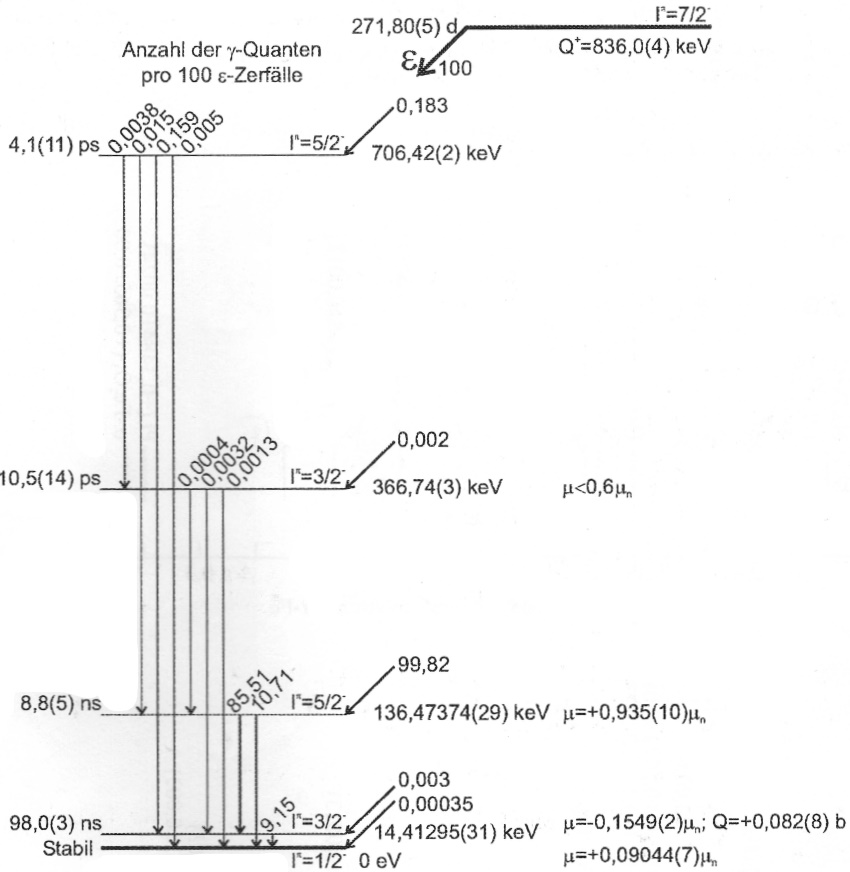
\includegraphics[width=0.9\linewidth]{img/Zerfallsschema}
	\caption{Zerfallsschema von $^{57}$Co.\cite{3}}
	\label{fig:zerfallsschema}
\end{figure}


\newpage


\section{Versuchsaufbau} \label{Aufbau}

Der Aufbau der Versuchsanordnung ist in Abbildung \ref{Versuchsaufbau} dargestellt und besteht im Wesentlichen aus einem Detektor (Proportionalzählrohr), einem sogenannten Mößbauer-Antrieb sowie einem Michelson-Interferometer.

\begin{figure}[H]
	\centering
	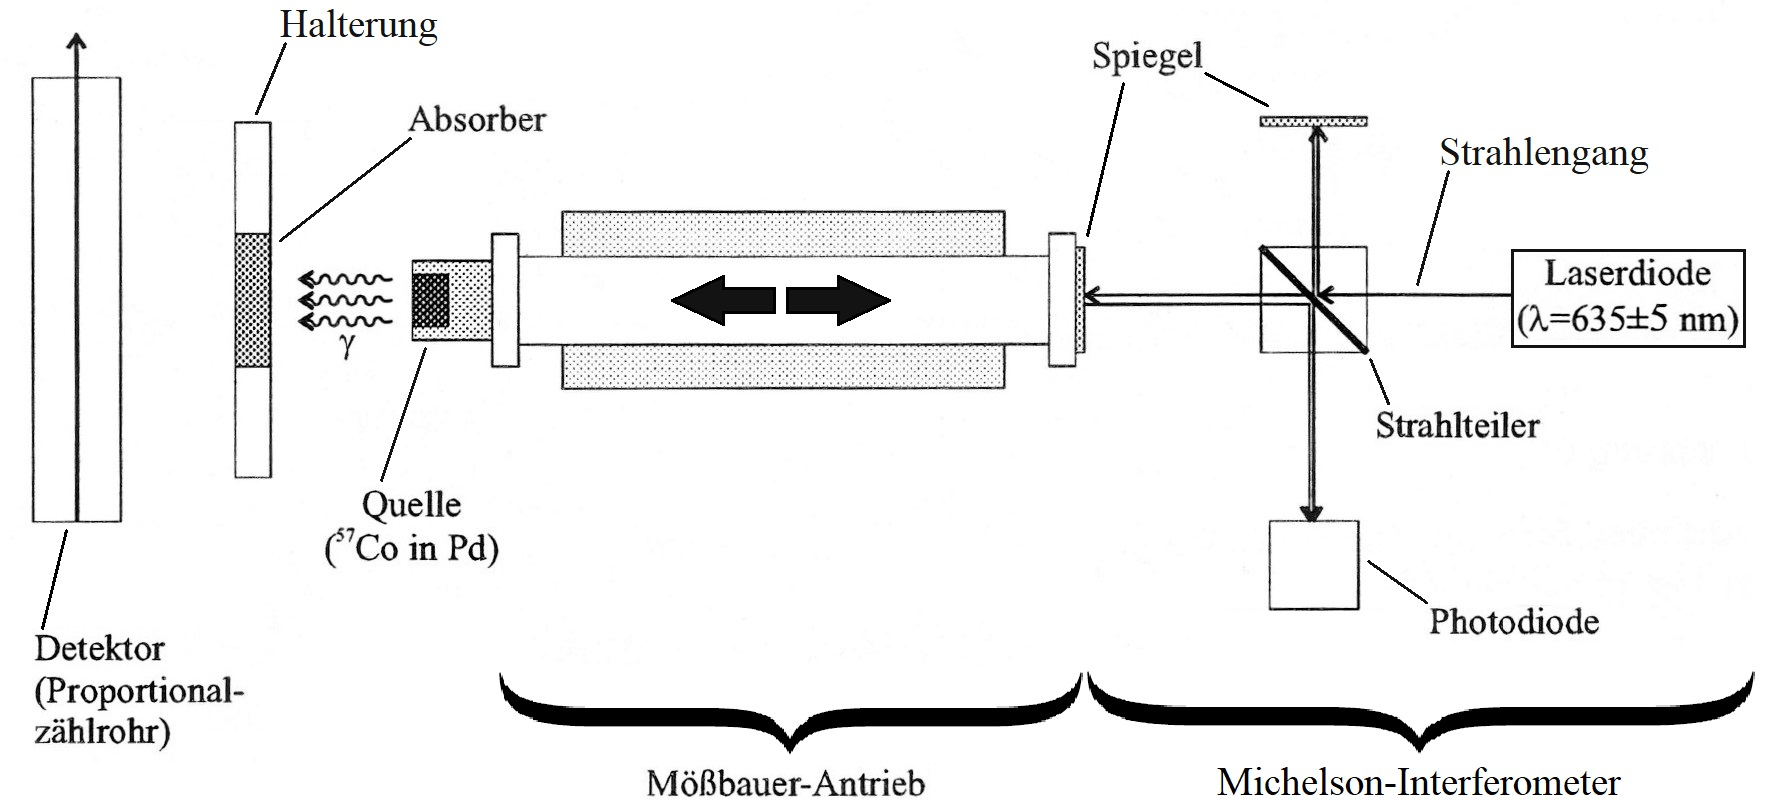
\includegraphics[width=1.0\textwidth]{img/VersuchsaufbauMoessbauer}
	\caption{Die Abbildung zeigt schematisch den Versuchsaufbau des Experiments zum Mößbauer-Effekt.\cite{4}}
	\label{Versuchsaufbau}
\end{figure}

\noindent Der Mößbauer-Antrieb vollführt eine kosinusförmige Bewegung in Richtung der in Abbildung \ref{Versuchsaufbau} eingezeichneten Pfeile.
Am linken Ende des Mößbauer-Antriebs ist eine $\gamma$-Strahlung emittierende Quelle befestigt, bei der es sich um in Palladium (Pd) eingebettetes Cobalt-$57$ ($^{57}$Co) handelt.
Diese $^{57}$Co-Probe besaß am \date{27.01.2015} eine Aktivität von $90\,$MBq.
Zwischen dem Proportionalzählrohr und der $\gamma$-Quelle befindet sich eine Halterung, in welche sich eine $\gamma$-Quanten absorbierende Probe einsetzen lässt.
Für die folgenden experimentellen Untersuchungen stehen drei verschiedene solcher Absorber A, B und C zur Verfügung, wobei ihre materielle Zusammensetzung unbekannt ist.

Das Proportionalzählrohr ist eine spezielle Verwendungsform eines Geiger-Müller-Zählrohrs.
Letzteres besteht aus einem an beiden Seiten verschlossenen, dünnen, zylindrischen Metallrohr, welches die Kathode bildet und mit einem Zählgas gefüllt ist.
Die Anode befindet sich in Form eines dünnen Drahts in der Symmetrieachse des Zylinders und wird an einem Ende durch einen Isolator aus dem Zählrohr herausgeführt.
Zwischen Kathode und Anode wird eine Gleichspannung angelegt und über einen elektrischen Widerstand die einfallende ionisierende Strahlung (hier: $\gamma$-Strahlung) gemessen.
Denn diese Strahlung erzeugt in der Gasfüllung freie Elektronen, welche im elektrischen Feld zur Anode wandern.
Beim Proportionalzählrohr wird die Gleichspannung nun so niedrig gehalten, dass keine selbständige Glimmentladung einsetzt.
Die Anzahl der Elektronen, die im hohen elektrischen Feld in der Umgebung des Zählrohrdrahtes durch Entladungsstoß gebildet werden, ist somit proportional zur Anzahl der primär erzeugten Ladungsträger.
Zudem ist der über den elektrischen Widerstand messbare Stromimpuls proportional zur Energie, welche die Strahlung im Zählrohr abgegeben hat, sodass das Proportionalzählrohr die Möglichkeit bietet, Teilchenenergien zu messen.

Einer der beiden Spiegel des Michelson-Interferometers ist am rechten Ende des Mößbauer-Antriebs angebracht.
Beim Michelson-Interferometer geschieht eine Aufteilung des von der Laserdiode mit der Wellenlänge $\lambda=(635\pm 5)\,$nm emittierten, kohärenten Laserstrahls mittels Strahlteiler.
Das transmittierte und das um $90\,$° reflektierte Laserlicht treffen jeweils auf einen vollständig reflektierenden Spiegel, werden auf den Strahlteiler zurückgeworfen und es wird wieder ein Teil des Laserlichts transmittiert und ein Teil um $90\,$° reflektiert.
Dieser Verlauf des Laserlichts wird am Strahlengang deutlich, welcher in Abbildung \ref{Versuchsaufbau} eingezeichnet ist.
Hinter dem Strahlteiler überlagern sich die elektromagnetischen Wellen der zwei Laserstahlen und es kommt zur Interferenz.
Verschiebt die Bewegung des Mößbauer-Antriebs den an dessen Ende angebrachten Spiegel, so verändert sich die optische Weglänge der dazugehörigen elektromagnetischen Welle und die Phasen der beiden elektromagnetischen Wellen verschieben sich gegeneinander.
Sind beide Wellen in Phase, spricht man von konstruktiver Interferenz.
Es handelt sich um destruktive Interferenz, wenn beide Wellen gegenphasig sind.
Die Wegdifferenz zwischen den Intensitätsmaxima (konstruktive Interferenz) zweier ebener Wellen gleicher Frequenz und Amplitude entspricht dem Gangunterschied.
Dieser beträgt wiederum ein ganzzahliges Vielfaches der Wellenlänge des verwendeten Laserlichts.
Also kann über eine Intensitätsmessung mit Hilfe der Photodiode die Bewegung des Mößbauer-Antriebs quantitativ erfasst werden.
Bewegt man nämlich den am rechten Ende des Mößbauer-Antriebs angebrachten Spiegel um die Wegstrecke $\Delta s$, so ändert sich die Helligkeit des Interferenzbildes periodisch.
Dieser Tatsache liegt folgender mathematischer Zusammenhang zwischen $\Delta s$, der Anzahl $N\in\mathbb{N}_{0}$ der beobachteten Intensitätsmaxima und der Wellenlänge $\lambda$ des verwendeten Lasergeräts zugrunde:

\begin{align}
\Delta s = N\cdot\frac{\lambda}{2}
\end{align}

\noindent Dabei kommt der Faktor $\frac{1}{2}$ dadurch zustande, dass der Laserstrahl aufgrund der Spiegelung im Michelson-Interferometer eine Gesamtstrecke von $2\Delta s$ zurücklegen muss.
Somit bildet $2\Delta s$ den Gangunterschied.


\newpage


\section{Durchführung}

Bei der Versuchsdurchführung wird zunächst an der Antriebselektronik des Mößbauer-Antriebs der Geschwindigkeitsbereich eingestellt, welchen es bei der Auswertung in Abschnitt \ref{AuswertungDiskussion} exakt zu ermitteln gilt.
Die Geschwindigkeit des Mößbauer-Antriebs wird sinusförmig mit einer Frequenz von $\nu = 24\,$Hz moduliert.
Da somit die $\gamma$-Quelle bewegt wird und es sich bei $\gamma$-Strahlung um elektromagnetische Strahlung handelt, findet, wie in Abschnitt \ref{Doppler} beschrieben, unter Ausnutzung des Doppler-Effekts eine Modulation der Energie über die Geschwindigkeit $v$ des Mößbauer-Antriebs statt.
Die Geschwindigkeit und damit die Energie der $\gamma$-Quanten wird durch die Zählung der Intensitätsmaxima des Michelson-Interferometers pro Zeitintervall gemessen.
Dazu wird jede $2\pi$-Periode der Sinusschwingung in $N_{K} = 512$ Zeitintervalle bzw. Kanäle zerlegt und in jedem Zeitintervall die Anzahl $N$ der Intensitätsmaxima registriert und somit die in diesem Zeitintervall zurückgelegte Wegstrecke gemessen.
Aus dem auf diese Weise bestimmten Weg und der Länge des Zeitintervalls ergibt sich die mittlere Geschwindigkeit in diesem Zeitintervall.
Die Wellenlänge $\lambda$ der Laserdiode, die Anzahl $N$ der beobachteten Intensitätsmaxima, die Anzahl $N_{K}$ der Zeitintervalle bzw. Kanäle pro $2\pi$-Periode, die Anzahl $N_\text{Runs}=20.000$ der vom Mößbauer-Antrieb pro Messung verrichteten Schwingungsperioden, die Frequenz $\nu$ und die Geschwindigkeit $v$ des Mößbauer-Antriebs unterliegen folgendem mathematischem Zusammenhang:

\begin{align} \label{KaliFormel}
v = \frac{\Delta s}{\Delta t} = \frac{\lambda N}{2}\cdot\frac{\nu N_{K}}{N_\text{Runs}}
\end{align}

\noindent Es existiert also eine Beziehung zwischen den Zeitintervallen bzw. Kanälen und der Geschwindigkeit $v$ des Mößbauer-Antriebs, welche wiederum mit der Energie der emittierten Photonen verknüpft ist.
Darüber hinaus liegt nach der Gleichung \ref{KaliFormel} zwischen $v$ und $N$ ein weiteres, sogar proportionales Verhältnis vor, zumal $\lambda$, $N_{K}$, $N_\text{Runs}$ und $\nu$ aufgrund der Gegebenheiten dieses Experiments Konstanten bilden.
Daraus resultiert, dass zwischen den Zeitintervallen bzw. Kanälen und der Anzahl $N$ der beobachteten Intensitätsmaxima ebenfalls eine Relation besteht.

Zunächst soll im Rahmen einer Kalibrierungsmessung für jeden der drei Absorber A, B und C die Relation zwischen den Kanälen und $N$ untersucht werden.
Dazu wird der entsprechende Absorber in die Halterung eingesetzt, die Photodiode über einen Analog-Digital-Wandler (Abkürzung: ADC) an einen Computer angeschlossen und die Messung des Kanalspektrums gestartet.
Dabei zählt die Elektronik der Photodiode die Intensitätsmaxima und addiert diese für jeden Kanal auf.
Die Elektronik des Mößbauer-Antriebs schaltet in gleichmäßigen Schritten durch die Kanäle und setzt den Zähler rechtzeitig zurück.

Bei der tatsächlichen Vermessung der Eigenschaften der Absorber A, B und C wird das Proportionalzählrohr zwecks Signalverstärkung an einen Verstärker (engl. \emph{Amplifier}) angeschlossen.
Das daraus stammende Signal wird mit einem Diskriminator auf den zu untersuchenden Bereich um $\SI{14,4}{\kilo\electronvolt}$ beschränkt und über einen Analog-Digital-Wandler an den Computer geleitet.
Dieser erhält also einerseits durch das Michelson-Interferometer die Information über die Kanäle und andererseits das Signal der Counts $N$ des Proportionalzählrohrs.
Der Grund für die Beschränkung auf den $\SI{14,4}{\kilo\electronvolt}$-Bereich ist unter anderem in Abschnitt \ref{ZerfallCobalt57} dargelegt und besteht darin, die Detektion anderer $\gamma$-Strahlung zu vermeiden.
Bei den drei Messungen A, B und C wird jeweils der entsprechende Absorber A, B bzw. C in die Halterung eingesetzt.
Anschließend wird mit Hilfe des Computers für jeden einzelnen der drei Absorber das Geschwindigkeitsspektrum aufgezeichnet.

Während des gesamten Experiments wird die Raumtemperatur $T$ im Labor überwacht und in Zeitabständen von ungefähr $15$ Minuten gemessen.


\newpage


\section{Auswertung und Diskussion} \label{AuswertungDiskussion}

Im Folgenden werden die Unsicherheiten sämtlicher Messdaten, Messwerte und Messergebnisse nach GUM\cite{1} bestimmt.
Für weitere Angaben wird an dieser Stelle auf den Anhang in Abschnitt \ref{Anhang} verwiesen.

\subsection{Messung A}

Im folgenden Abschnitt soll der Absorber A analysiert werden.

\subsubsection{Kalibrierung} \label{KaliMessungA}

Zunächst werden die im Zuge der Kalibrierungsmessung für den Absorber A erhaltenen Daten des Kanalspektrums einer FFT (engl. \emph{Fast Fourier Transform}) und einer Bandpassfilterung um $\SI{24}{\hertz}$ unterzogen, damit die Genauigkeit der Kalibrierung steigt und es zu einer Verbesserung der weiteren Analyse kommt.
Dadurch wird nämlich das Spektrum geglättet und die Erstellung einer Anpassungskurve begünstigt, sodass sich die Unsicherheiten der Fitparameter verringern.
Aufgrund der sinusförmigen Modulation der Auslenkung des Mößbauer-Antriebs wird jede Geschwindigkeit in einer $2\pi$-Periode doppelt durchfahren.
Daher weisen sämtliche gemessenen Spektren eine Spiegelung um den Kanal $256$ auf.
Um die Spiegelung zu beseitigen, wird die Anzahl der Kanäle auf $\frac{512}{2}=256$ reduziert.
Dementsprechend werden die $512$ gemessenen Werte für die Anzahl $N$ der beobachteten Intensitätsmaxima angepasst und gemäß der Vorschrift

\begin{align}
N_{i}^{\text{(neu)}} = N_{257-i} + N_{256+i} \ \ , \ \ \ \ i=1,\dotsc ,256
\end{align}

\noindent iterativ übereinander gelegt.
Mithilfe der Formel \ref{KaliFormel} lassen sich die daraus erhaltenen $256$ (neuen) $N$-Werte jeweils in eine Geschwindigkeit $v$ umrechnen.
Bei diesen $v$-Werten muss es sich um betragsmäßige Geschwindigkeiten handeln, weil sie stets positiv sind und der Mößbauer-Antrieb eigentlich eine Hin-und-Her-Bewegung vollführt.
Trägt man die als $|v|$ zu interpretierenden Geschwindigkeitswerte gegen die $256$ Kanäle auf, so ergibt sich das in Abbildung \ref{KanalspektrumA} dargestellte, geglättete und von der Spiegelung bereinigte Kanalspektrum.

\begin{figure}[H]
	\centering
	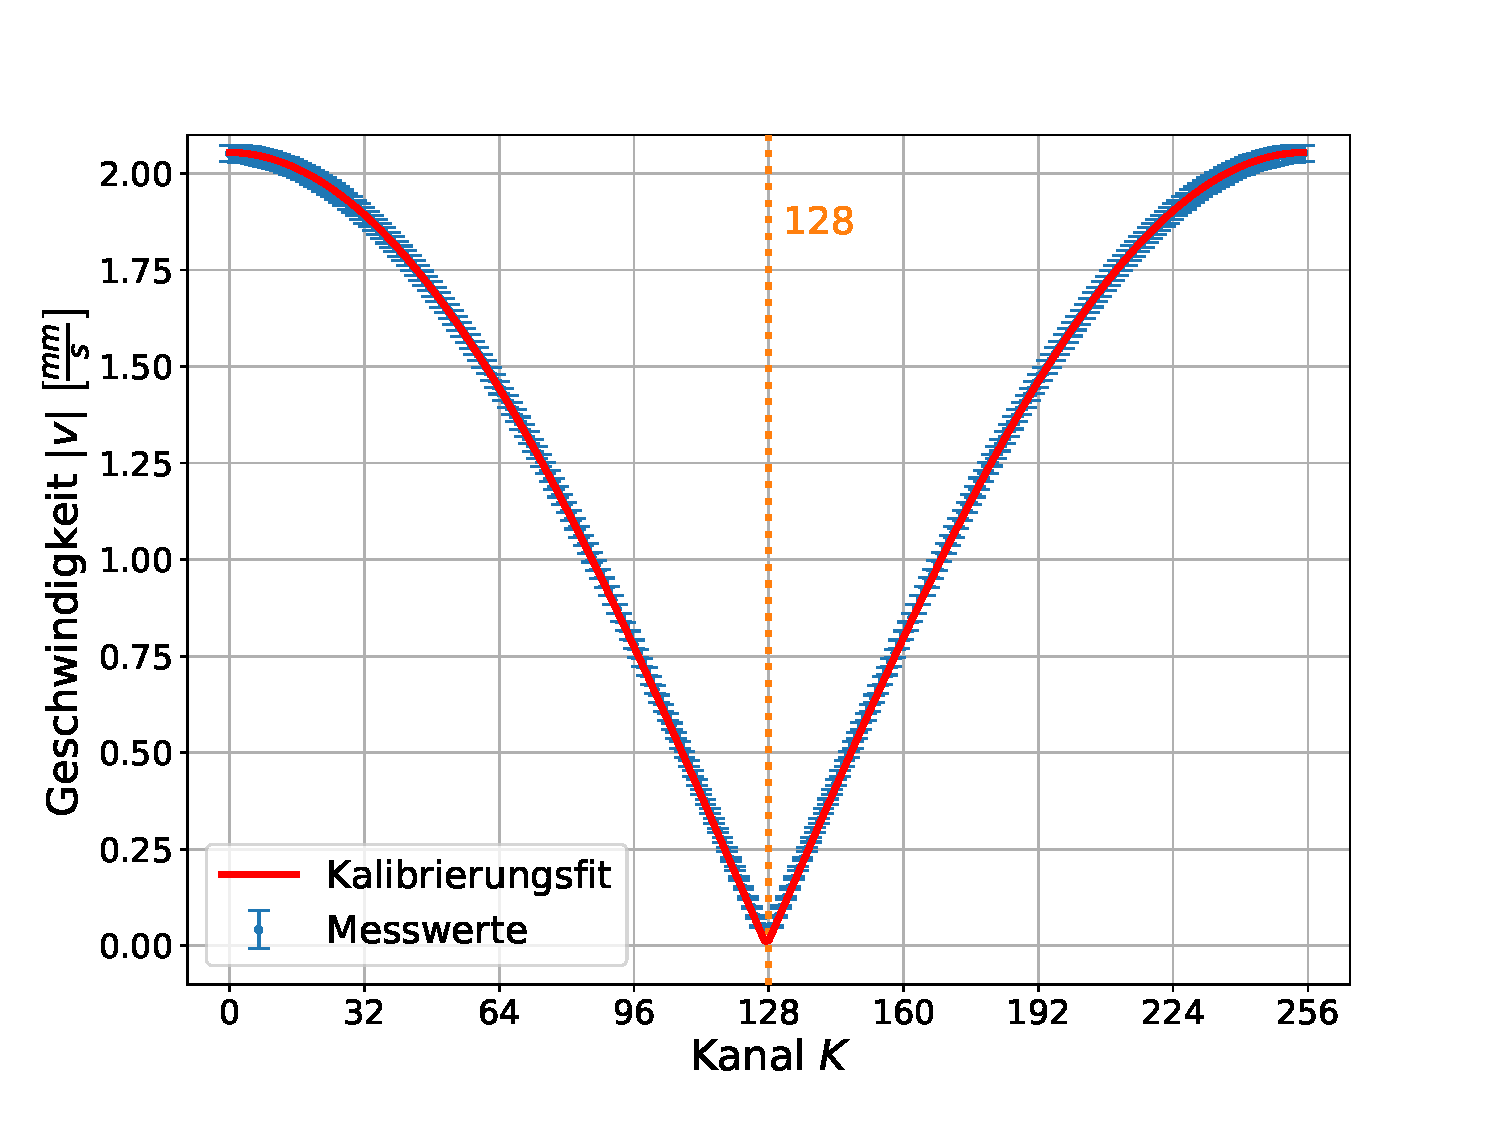
\includegraphics[width=0.8\textwidth]{raw/KanalspektrumA}
	\caption{Die Abbildung zeigt das im Rahmen der Kalibrierungsmessung für den Absorber A erhaltene und von der Spiegelung bereinigte Kanalspektrum, welches einer FFT (engl. \emph{Fast Fourier Transform}) und einer Bandpassfilterung um $\SI{24}{\hertz}$ unterzogen wurde. Zusätzlich ist der Kalibrierungsfit mit den Fitparametern $A=(2,0551\pm 0,0005)\,\frac{\textnormal{mm}}{\textnormal{s}}$ und $\varphi=0,50\pm 0,02$ zu sehen.}
	\label{KanalspektrumA}
\end{figure}

\noindent Nun lässt sich eine Anpassungskurve, die eine (ko-)sinusförmige Bewegung beschreibt und die Gestalt

\begin{align} \label{KaliFit}
f(x)=A\cdot\left|\cos\left(\frac{\pi}{256}\cdot (x+\varphi)\right)\right| 
\end{align}

\noindent besitzt, an die Messwerte fitten.
Die Werte für die Fitparameter dieses Kalibrierungsfits sind der Bildunterschrift der Abbildung \ref{KanalspektrumA} zu entnehmen. 
Mit Verzicht auf den Betragscharakter der Gleichung \ref{KaliFit} ergibt sich der folgende funktionale Zusammenhang zwischen der Geschwindigkeit $v$ und den Kanälen $K$:

\begin{align} \label{ChanelToVelocity}
v(K)=A\cdot\cos\left(\frac{\pi}{256}\cdot (K+\varphi)\right)
\end{align}

\noindent Hierbei kann das Vorzeichen beliebig gewählt werden.


\subsubsection{Bestimmung der Isomerieverschiebung} \label{v_isoA}

Im Folgenden soll anhand der gemessenen Isomerieverschiebung des Absorbers A auf dessen materielle Zusammensetzung geschlossen werden.
Dafür wird zunächst bei den aus der Messung A erhaltenen Daten des Geschwindigkeitsspektrums die Spiegelung nach dem gleichen Verfahren wie in Abschnitt \ref{KaliMessungA} beseitigt.
Anschließend werden die daraus hervorgehenden $256$ Kanäle mit Hilfe der Formel \ref{ChanelToVelocity} als Geschwindigkeit $v$ ausgedrückt.
Auf Basis dieser Kalibrierungsmethode ergibt sich das in Abbildung \ref{GeschwindigkeitsspektrumA} dargestellte Geschwindigkeitsspektrum.

\begin{figure}[H]
	\centering
	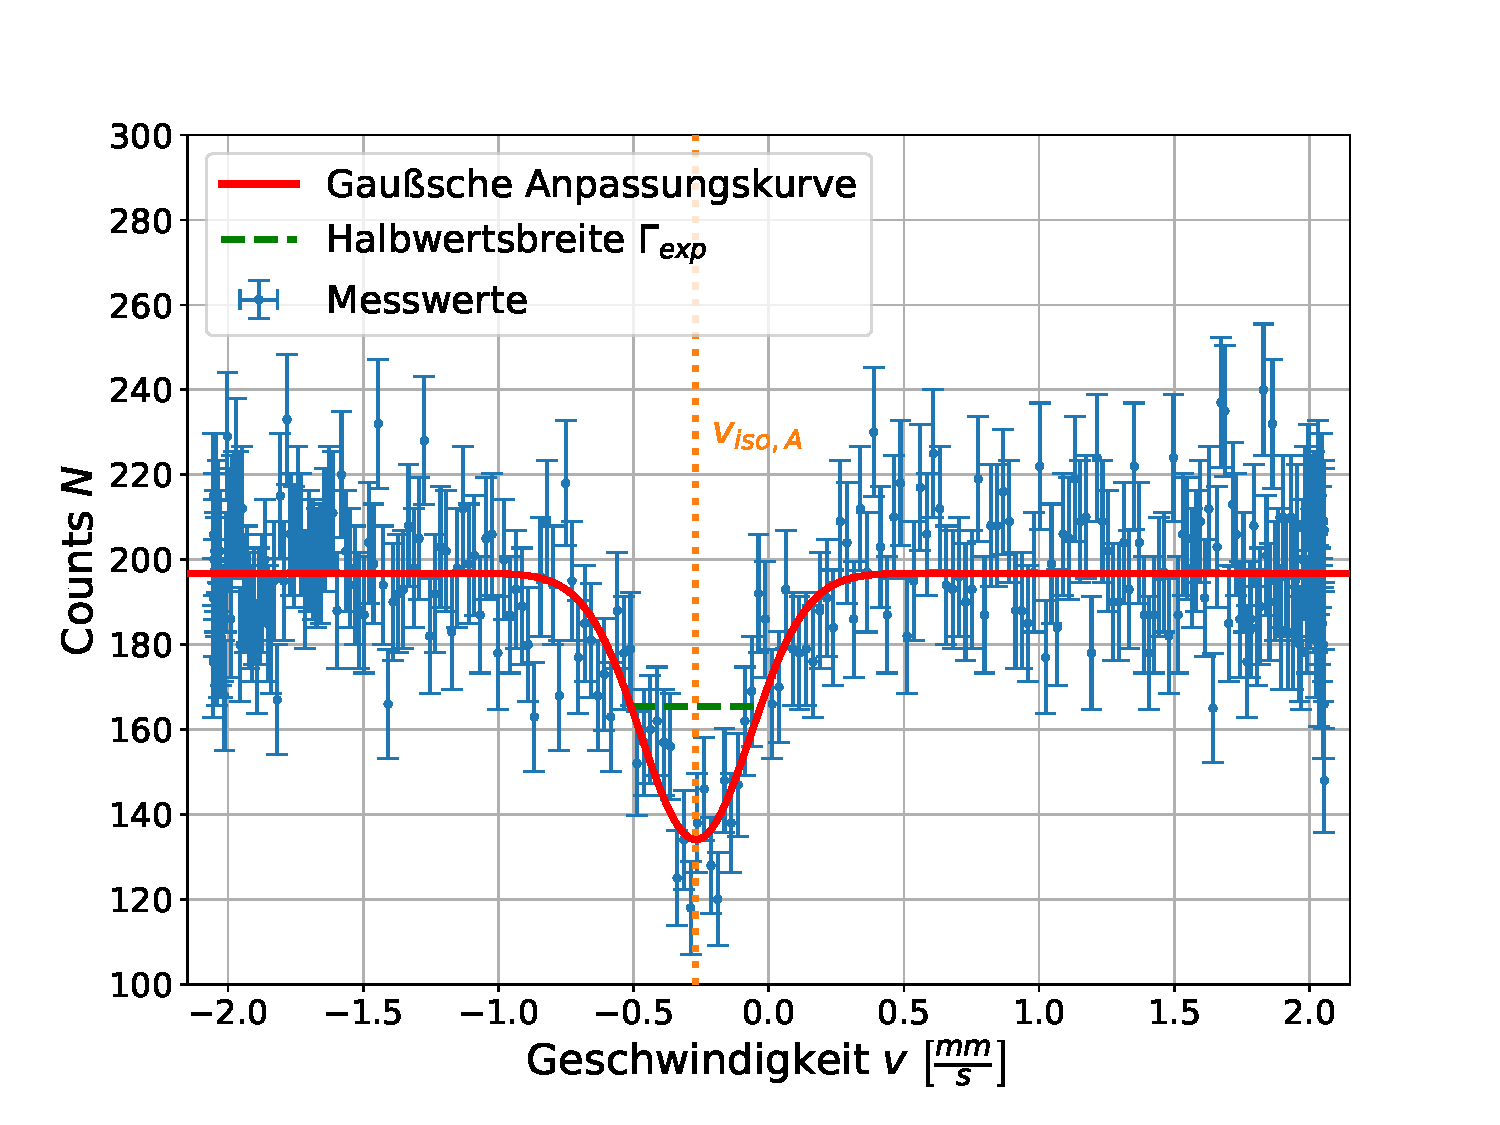
\includegraphics[width=0.8\textwidth]{raw/GeschwindigkeitsspektrumA}
	\caption{Die Abbildung zeigt das bei der Messung A bzw. mit dem Absorber A aufgenommene Geschwindigkeitsspektrum. Darüber hinaus ist die gaußsche Anpassungskurve und die Halbwertsbreite zu sehen. Die Position der Gauß-Kurve bzw. die Isomerieverschiebung ist mit einer orangefarbenen, gepunkteten, vertikalen Linie gekennzeichnet.}
	\label{GeschwindigkeitsspektrumA}
\end{figure}

\noindent Betrachtet man nun die Verteilung der Messwerte in diesem Geschwindigkeitsspektrum, so erscheint es naheliegend, eine gaußsche Anpassungskurve der Form

\begin{align}
f(x)=A\cdot\exp\left( -\frac{(x-\mu)^2}{2\sigma ^2}\right) +B
\end{align}

\noindent anzufitten.
Die Erstellung dieses Gauß-Fits, welcher im Geschwindigkeitsspektrum in Abbildung \ref{GeschwindigkeitsspektrumA} zu sehen ist, liefert folgende Werte für die Fitparameter:

\begin{align*}
A &= -62,7\pm 4,1 \\
\mu &=  (-0,270\pm 0,016)\,\frac{\textnormal{mm}}{\textnormal{s}} \\
\sigma &= (0,203\pm 0,017)\,\frac{\textnormal{mm}}{\textnormal{s}} \\
B &= 196,8\pm 1,0
\end{align*}

\noindent Die Position $\mu$ der Gauß-Kurve entspricht dabei der Isomerieverschiebung $v_\text{iso}$, die zudem im Geschwindigkeitsspektrum mit einer orangefarbenen, gepunkteten, vertikalen Linie markiert ist.
Mit $v_\text{iso} = \mu$ und unter Berücksichtigung des $\pm 1\sigma$-Bereichs des $v_\text{iso}$- bzw. $\mu$-Werts lässt sich das Material des Absorbers A als Edelstahl identifizieren, welches nach Abbildung \ref{fig:isoVgl} eine Isomerieverschiebung relativ zu $^{57}$Fe in Pd von $(-0,2658\pm 0,0032)\,\frac{\textnormal{mm}}{\textnormal{s}}$ aufweist.


\subsubsection{Berechnung des Messeffekts}

Der in diesem Abschnitt zu bestimmende Messeffekt für die Messung A ist als

\begin{align}
\frac{Z(\infty)-Z(v_\text{R})}{Z(\infty)}=\frac{B-(B+A)}{B}=-\frac{A}{B}>0
\end{align}

\noindent definiert, wobei $Z(v_\text{R})=Z(v_\text{iso})$ die Zählrate im Resonanzfall und $Z(\infty)$ die Zählrate weit außerhalb des Resonanzfalls bildet.
Dieser Gleichung liegt die Tatsache zugrunde, dass sich die beiden Zählraten über die Fitparameter der im Geschwindigkeitsspektrum in Abbildung \ref{GeschwindigkeitsspektrumA} dargestellten gaußschen Anpassungskurve ausdrücken lassen.
Denn es gilt $Z(v_\text{R})=B+A$ und $Z(\infty)=B$ mit $B>0$, $A<0$.
Mithilfe der $A$- und $B$-Werte aus Abschnitt \ref{v_isoA} erhält man schließlich den Messeffekt:

\begin{align*}
-\frac{A}{B}=(31,9\pm 2,1)\,\textnormal{\%}
\end{align*}


\subsubsection{Gemessene und theoretische Halbwertsbreite}

Das in Abbildung \ref{RaumtemperaturLabor} dargestellte $t$-$T$-Diagramm zeigt, wie sich die in Kelvin (K) angegebene Raumtemperatur $T$ im Labor während des gesamten Experiments entwickelt.

\begin{figure}[H]
	\centering
	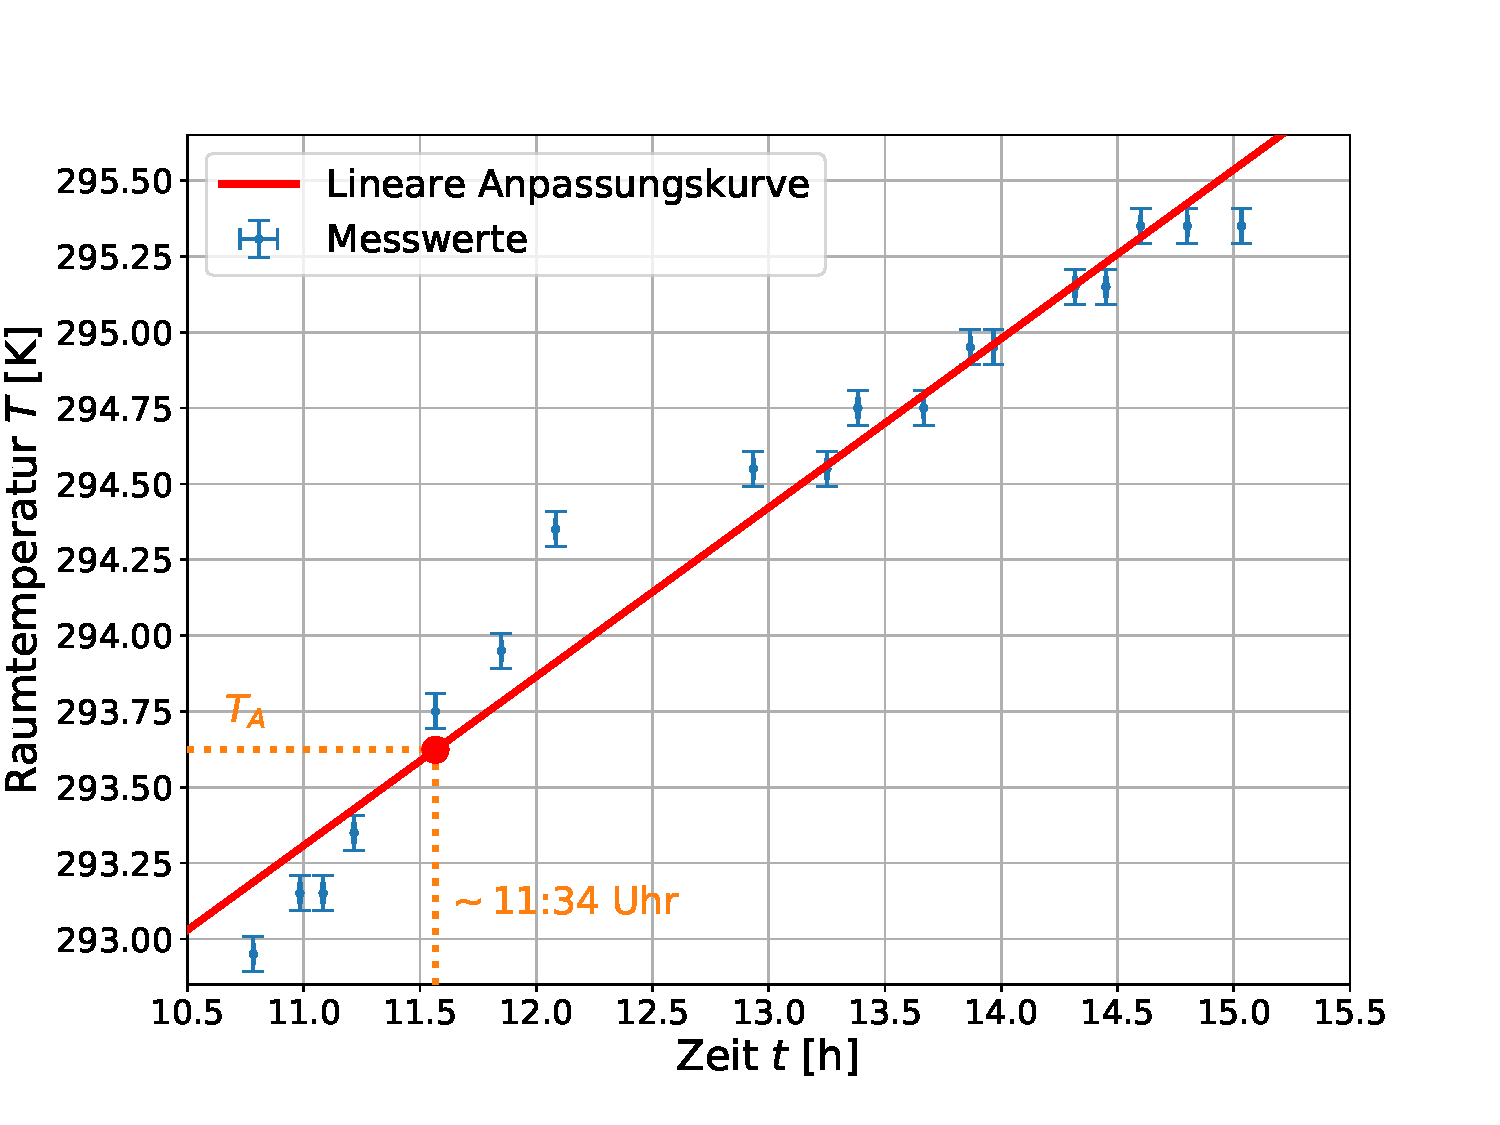
\includegraphics[width=0.8\textwidth]{raw/RaumtemperaturLabor}
	\caption{Das in dieser Abbildung dargestellte $t$-$T$-Diagramm veranschaulicht die Entwicklung der Raumtemperatur $T$ im Labor während des gesamten Experiments. Dem Verlauf der linearen Anpassungskurve entsprechend herrschte zu Beginn der Messung A um 11:34 Uhr eine Raumtemperatur von $T_{A}=(20,5\pm 0,5)\,$°C.}
	\label{RaumtemperaturLabor}
\end{figure}

\noindent Es ist ein annähernd linearer Zusammenhang zwischen $T$ und der Uhrzeit $t$ zu erkennen, sodass sich eine lineare Anpassungskurve der Form

\begin{align}
T(t) = m\cdot t + n
\end{align}

\noindent in das $t$-$T$-Diagramm einfügen lässt.
Anhand dieser Geraden kann man die Raumtemperatur zu Beginn der Messung A um 11:34 Uhr auf $T_{A}=(293,6\pm 0,5)\,$K abschätzen.
Nach der Gleichung

\begin{align}
\begin{split}
\Gamma_{korr}=\Big( &2,02+0,29\cdot f_{A}(T,\Theta_{D})\cdot\sigma_{0}\cdot\eta\cdot n\cdot d \\ %Oder: \nonumber \\ % no number is shown in this line
&-0,005\cdot\left( f_{A}(T,\Theta_{D})\cdot\sigma_{0}\cdot\eta\cdot n\cdot d\right) ^2 \Big)\cdot\Gamma_{nat}
\end{split}
\end{align}

\noindent wird nun die theoretisch vorhergesagte Halbwertsbreite $\Gamma_{korr}$ berechnet.
Dabei ist $f_{A}(T,\Theta_{D})$ der in Abschnitt \ref{DebyeWaller} erwähnte Debye-Waller-Faktor, $T=T_{A}$ die Raumtemperatur zu Beginn der Messung A, $\sigma_{0}$ der Streuquerschnitt, $\eta$ die Isotopenhäufigkeit von $^{57}$Fe in natürlichem Eisen, $n$ die Anzahl der Fe-Atome pro Kubikzentimeter, $\rho$ die Dichte von Edelstahl, $M_{\textnormal{Fe}}$ die mittlere Atommasse von natürlichem Eisen, $d$ die Dicke des Absorbers, $\Gamma_{nat}$ die natürliche Linienbreite der $14,4\,$keV-$\gamma$-Linie, $\Theta_{D}$ die Debye-Temperatur, $\hbar k$ der Impuls des $\gamma$-Quants, $M$ die Masse eines $^{57}$Fe-Atoms und $k_{B}$ die Boltzmann-Konstante.
Da aus Abschnitt \ref{v_isoA} bekannt ist, dass es sich beim Absorber A um Edelstahl handelt, werden bei der Berechnung von $\Gamma_{korr}$ folgende eisen- und edelstahlspezifische Konstanten verwendet:

\begin{align*}
\sigma_{0} &= 2,38\cdot 10^{-18}\,\textnormal{cm}^2 \\
\eta &= 0,0219 \\
n &= \frac{\rho}{M_{\textnormal{Fe}}} \\
\rho &= 0,0079\,\frac{\textnormal{kg}}{\textnormal{cm}^3} \\
M_{\textnormal{Fe}} &= 56,845\,\textnormal{u} \\
d &= 25\,\mu\textnormal{m} \\
\Gamma_{nat} &= 0,097\,\frac{\textnormal{mm}}{\textnormal{s}} \\
\Theta_{D} &= 450\,\textnormal{K} \\
\hbar k &= \frac{E_{\gamma}}{c}=14,41295\,\frac{\textnormal{keV}}{\textnormal{c}} \\
M &= 56,935398\,\textnormal{u} \\
k_{B} &= 8,617342\cdot 10^{-5}\,\frac{\textnormal{eV}}{\textnormal{K}} \\
1\,\textnormal{u} &= 931,494013\,\frac{\textnormal{MeV}}{\textnormal{c}^2}
\end{align*}

\noindent Für die Messunsicherheit der theoretischen Halbwertsbreite reicht es aus, wenn nur die Unsicherheit des Raumtemperaturwerts $T_{A}$ berücksichtigt wird.

Die Halbwertsbreite (FWHM) einer wie in Abbildung \ref{GeschwindigkeitsspektrumA} dargestellten Gauß-Kurve mit der Breite $\sigma$ ist als

\begin{align}
\textnormal{FWHM}=2\sqrt{2\ln (2)}\cdot\sigma
\end{align}

\noindent definiert.
Für die experimentell bestimmte bzw. gemessene Halbwertsbreite $\Gamma_{exp}$ gilt dementsprechend:

\begin{align}
\Gamma_{exp}=2\sqrt{2\ln (2)}\cdot\sigma
\end{align}

\noindent Unter Verwendung dieser Formel und des in Abschnitt \ref{v_isoA} ermittelten Fitparameters $\sigma$ erhält man somit einen Wert für die gemessene Halbwertsbreite $\Gamma_{exp}$, welche zudem im Geschwindigkeitsspektrum in Abbildung \ref{GeschwindigkeitsspektrumA} veranschaulicht ist.

Insgesamt lauten die Werte der theoretischen und der gemessenen Halbwertsbreite:

\begin{align*}
\Gamma_{korr} &= (0,39353\pm 0,00012)\,\frac{\textnormal{mm}}{\textnormal{s}} \\
\Gamma_{exp} &= (0,48\pm 0,04)\,\frac{\textnormal{mm}}{\textnormal{s}}
\end{align*}

\noindent Es zeigt sich, dass die Halbwertsbreiten $\Gamma_{korr}$ und $\Gamma_{exp}$ zwar die gleiche Größenordnung besitzen, jedoch im Rahmen ihrer jeweiligen $\pm 1\sigma$-Bereiche nicht übereinstimmen.
Ein Grund dafür könnte die Tatsache sein, dass die bei diesem Experiment vorausgesetzten Modellannahmen der Theorie zu keiner exakten Widerspiegelung der Realität führen.
Ein weiterer Grund könnte die Existenz eines unbekannten und daher nicht berücksichtigten Fehlers in der Versuchsanordnung sein, sodass eine Messung mit einer präziseren Apparatur erforderlich ist.


\subsubsection{Relative Änderung des Kernladungsradius $\Delta R/R$ von $^{57}$Fe} \label{A:dRR}

Um die relative Änderung des Kernladungsradius $\frac{\Delta R}{R}$ zwischen dem Grundzustand und dem $14,4\,$keV-Niveau des $^{57}$Fe zu bestimmen, formt man die Gleichung \ref{relAenderungKernladungsradius} aus Abschnitt \ref{Doppler} nach

\begin{align} \label{eq:dRR_A}
\frac{\Delta R}{R}=\frac{5\varepsilon_{0}E_{\gamma}}{S^{\prime}(Z)ce^{2}ZR^2\left( \left| \Psi_\text{ss}(0)\right|^2 - \left| \Psi_\text{Pd}(0)\right|^2\right)}\cdot v_\text{iso}
\end{align}

\noindent um.
Dabei ist $E_{\gamma}$ die Energie des $\gamma$-Quants, $Z$ die Kernladungszahl, $S^{\prime}(Z)$ ein relativistischer Korrekturfaktor, $R$ der Kernradius, $A$ die Massenzahl, $\left| \Psi_\text{A}(0)\right|^2 = \left| \Psi_\text{ss}(0)\right|^2$ die Elektronendichte am Kernort von $^{57}$Fe in Edelstahl, $\left| \Psi_\text{Q}(0)\right|^2 = \left| \Psi_\text{Pd}(0)\right|^2$ die Elektronendichte am Kernort von $^{57}$Fe in Palladium und $a_{0}$ der bohrsche Radius.
Da aus Abschnitt \ref{v_isoA} bekannt ist, dass es sich beim Absorber A um Edelstahl und bei der Quelle um $^{57}$Fe in Palladium handelt, setzt man folgende Konstanten in Gleichung \ref{eq:dRR_A} ein:

\begin{align*}
E_{\gamma} &= 14,41295\,\textnormal{keV} \\
Z &= 26 \\
S^{\prime}(Z=26) &= 1,33 \\
R &= \sqrt[3]{A}\cdot 1,3\,\textnormal{fm} \\
A &= 57 \\
a_{0} &= 0,0529\,\textnormal{nm} \\
\left| \Psi_\text{ss}(0)\right|^2 &= 11.882,4\cdot a_{0}^{-3} \\
\left| \Psi_\text{Pd}(0)\right|^2 &= 11.881,8\cdot a_{0}^{-3}
\end{align*}

\noindent Zusätzlich verwendet man die für den Absorber A bestimmte Isomerieverschiebung $v_\text{iso}$, sodass man für die relative Änderung des Kernladungsradius schließlich

\begin{align*}
\frac{\Delta R}{R}=(-0,102\pm 0,006)\,\textnormal{\%}
\end{align*}

\noindent erhält.
Dies bedeutet, dass die absolute Änderung des Kernladungsradius relativ zur Kerngröße sehr gering ist.
Außerdem spricht das Vorzeichen des $\frac{\Delta R}{R}$-Werts für eine Verkleinerung, was letztendlich darauf hinweist, dass der $^{57}$Fe-Kern beim Übergang vom $14,4\,$keV-Niveau in den Grundzustand nicht wesentlich kleiner wird.


\subsection{Messung B}

Im folgenden Abschnitt soll der Absorber B analysiert und die elektrische Quadrupolaufspaltung im Kern gezeigt werden.
Dazu wird der elektrische Feldgradient in $z$-Achse berechnet.
Der Auswertung in diesem Abschnitt liegt die in Abbildung \ref{fig:velocityB} zu sehende Kalibrierung zugrunde.
Die Entstehung dieser Kalibrierungsmessung basiert auf einer Methodik, welche analog zu der in Abschnitt \ref{KaliMessungA} Beschriebenen ist.

\begin{figure}[H]
	\centering
	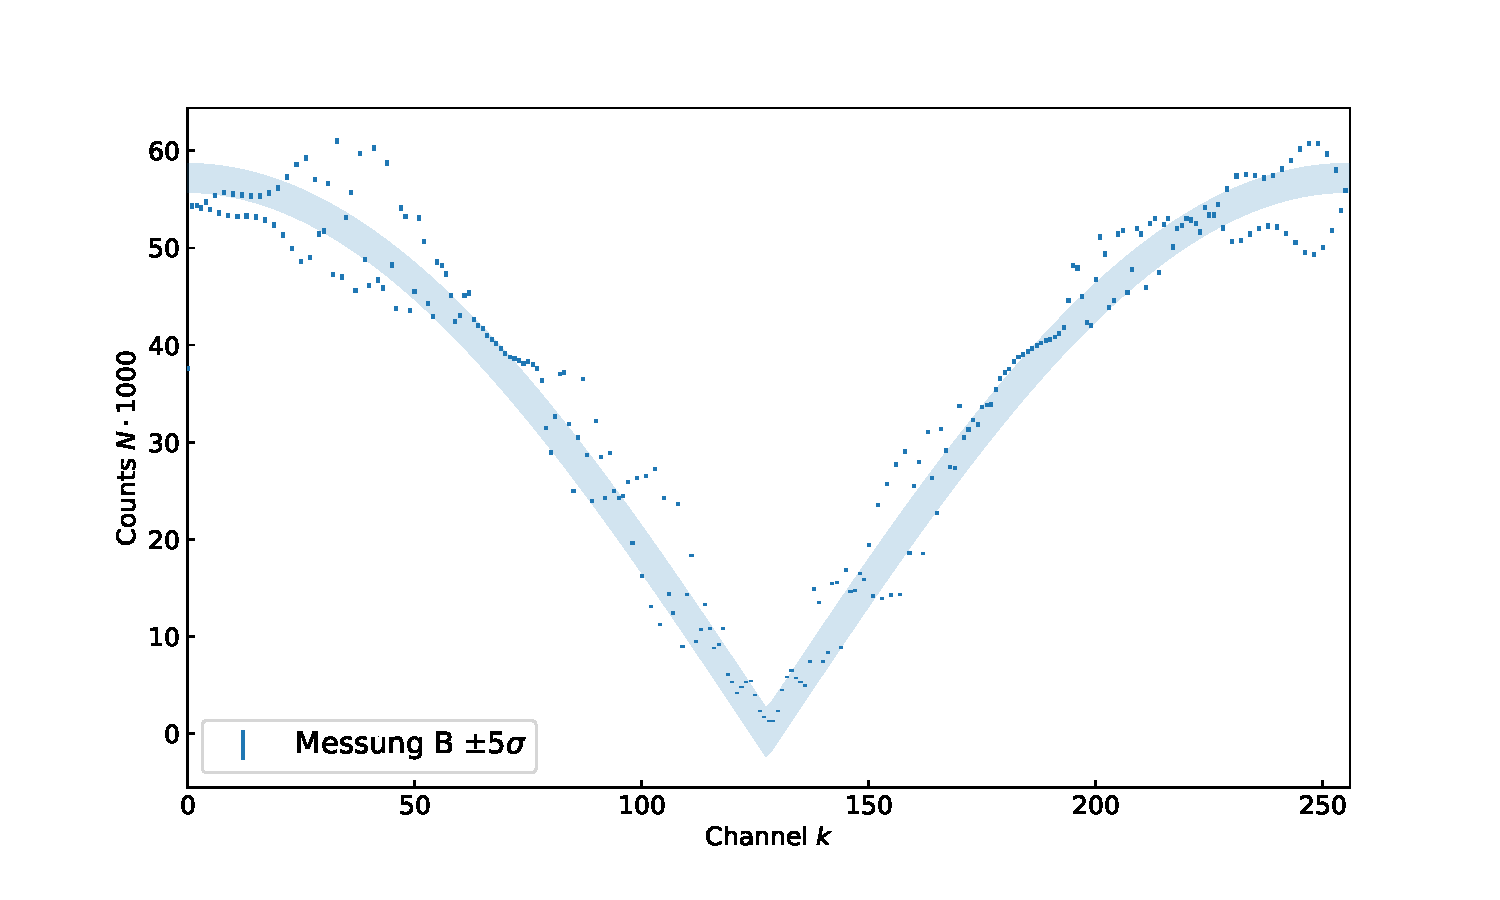
\includegraphics[width=1.0\textwidth]{dat/velocityB.pdf}
	\caption{Kalibrierung für die Messung B. Eingezeichnet sind die ungefilterten Messwerte und die Fitfunktion mit den Fitparametern $A = (5,721 \pm 0,030) \cdot 10^4$ und $\varphi=0,4 \pm 0,7$.}
	\label{fig:velocityB}
\end{figure}

\noindent Die Amplitude dieser Kalibrierungsmessung liegt deutlich über jener der anderen Messungen.
Dies könnte an einer geringeren Masse des Absorbers B liegen.


\subsubsection{Isomerieverschiebung}

Um die Isomerieverschiebung zu erhalten, wird das Spektrum der durch den Absorber B transmittierten Strahlung gemessen.
Das sich dabei ergebene Geschwindigkeitsspektrum ist in Abbildung \ref{fig:IsomerieB} zu sehen.
Bei dieser Messung des Spektrums wurde die Intensität über $40.000$ Iterationen addiert, um eine größere Statistik zu erhalten.

\begin{figure}[H]
	\centering	
	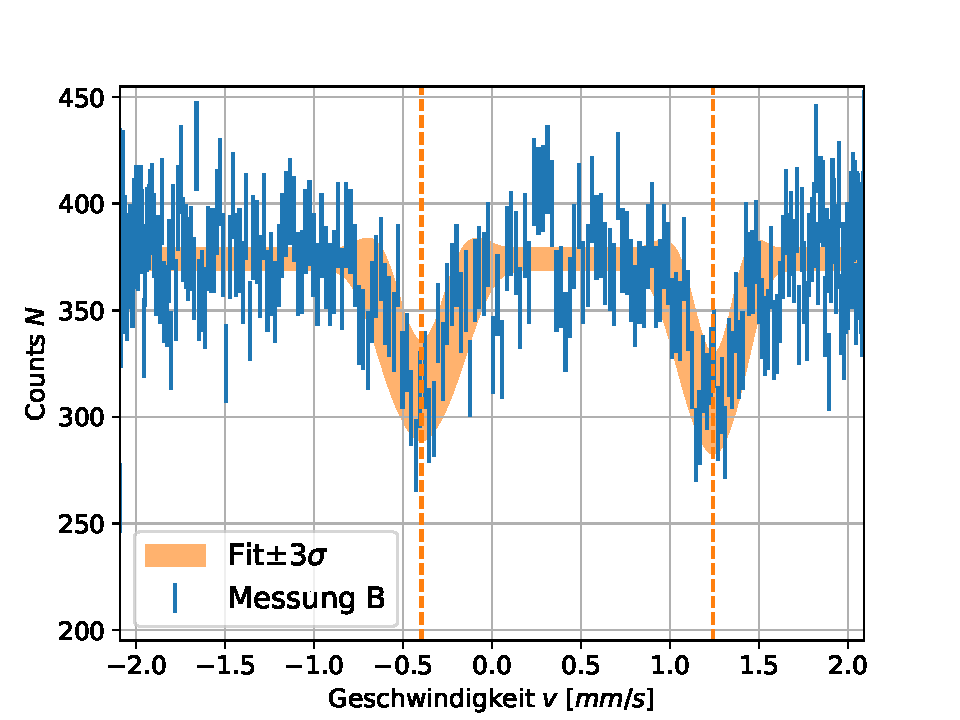
\includegraphics[width=0.95\textwidth]{dat/messungB.pdf}	
	\caption{Die Abbildung zeigt das bei der Messung B bzw. mit dem Absorber B aufgenommene Geschwindigkeitsspektrum. Es ist ein Gauß-Fit mit zwei Peaks eingezeichnet. Die Positionen der Peaks sind der Tabelle \ref{tab:isoB} zu entnehmen. Aus dem Mittelwert beider Peaks ergibt sich $v_\text{iso,B}=\protect\input{dat/messungB_iso.txt}$.}
	\label{fig:IsomerieB}
\end{figure}

\noindent Da die Aufspaltung durch elektrische Quadrupolwechselwirkung gleichmäßig ist, kann hier die Isomerieverschiebung durch Mittelung beider Peakpositionen auf

\begin{align*}
v_\text{iso, B} = \frac{v_1 + v_2}{2} = \input{dat/messungB_iso.txt}
\end{align*}

\noindent ermittelt werden.
Damit lässt sich das Material des Absorbers B als $Na_2Fe(CN)_5NO \cdot 2H_2O$ identifizieren, welches nach Abbildung \ref{fig:isoVgl} eine Isomerieverschiebung relativ zu $^{57}$Fe in Pd von $\SI{-0.4374 \pm 0.0018}{\milli\meter\per\second}$ aufweist.

Die entsprechenden Aufspaltungsenergien beider Zustände können in Tabelle \ref{tab:isoB} abgelesen werden.
Sie ist definiert als die Differenz der Anregungsenergie und der Isomerieverschiebung.

\begin{table}[H]
	\centering
	\caption{Energieaufspaltungen beider Peaks von Absorber B.} 
	\label{tab:isoB}
	\begin{tabular}{c|ccc}
		\toprule
		&       $v_\text{res}$         &     $\Delta v_\text{iso}$      &     $\Delta E_\text{iso}$     \\ \midrule
		Peak 1 & \input{dat/messungB_x_1.txt} & \input{dat/messungB_v_1.txt} & \input{dat/messungB_E_1.txt}  \\
		Peak 2 & \input{dat/messungB_x_0.txt} & \input{dat/messungB_v_0.txt} & \input{dat/messungB_E_0.txt}  \\ \bottomrule
	\end{tabular}
\end{table}


\subsubsection{Elektronendichte}

Um die Elektronendichte $\abs{\Psi_\text{A}(0)}^2$ des Absorbers im Kern zu ermitteln, wird Gleichung \ref{relAenderungKernladungsradius} nach

\begin{align}
\abs{\Psi_\text{A}(0)}^2 = \frac{5 v_\text{iso} E_\gamma \varepsilon_0}{S'(Z = 26) c e^2 Z R^2}\cdot\left( \frac{\Delta R}{R}\right) ^{-1} + \abs{\Psi_\text{Q}(0)}^2 = \input{dat/electrondensity_B.txt}
\end{align}

\noindent umgestellt.
Dabei ist $\frac{\Delta R}{R}=(0,102\pm 0,006)\,$\% aus Abschnitt \ref{A:dRR} bekannt und die Elektronendichte $\abs{\Psi_\text{Q}(0)}^2 = \SI{11881,8}{a_0^{-3}}$ von $^57$Fe in Pd gegeben.
Weiter sind $E_\gamma = \SI{14,4}{keV}$ die Quellphotonenenergie, $Z=26$ die Ordnungszahl von Eisen, $S'(Z = 26) = 1,33$ der relativistische Korrekturfaktor von Eisen und $R=\sqrt[3]{A}\cdot 1,3\,$fm der Kernradius mit $A=57$ für Eisen.


\subsubsection{Elektrischer Feldstärkegradient}

Da die Aufspaltung in Abbildung \ref{fig:IsomerieB} auf ein elektrisches Quadrupolmoment zurückzuführen ist, kann mit der Aufspaltungsenergie der Gradient des elektrischen Feldstärketensors in $z$-Richtung

\begin{align}
V_{zz} = \frac{2 \Delta E}{e Q} = \input{dat/Vzz_B.txt}
\end{align}

\noindent bestimmt werden.
Hierbei ist $\Delta E = \input{dat/messungB_dv.txt}$ die Aufspaltung zwischen den beiden Peaks und $Q = \SI{0,082 \pm 0,008}{b}$ das elektrische Quadrupolmoment von $^{57}$Co
Da es sich bei Atomkernen um sehr kleine Längenskalen handelt, ist dementsprechend auch das elektrische Feld sehr hoch und fällt ebenso schnell ab.


\subsection{Messung C}

Im folgenden Abschnitt soll der Absorber C analysiert und die magnetische Aufspaltung im Kern gezeigt werden.
Hierzu wird das magnetische Moment des angeregten Zustands und das Magnetfeld im Kern bestimmt.
Der Auswertung in diesem Abschnitt liegt die in Abbildung \ref{fig:velocityC} zu sehende Kalibrierung zugrunde.
Die Entstehung dieser Kalibrierungsmessung basiert auf einer Methodik, welche analog zu der in Abschnitt \ref{KaliMessungA} Beschriebenen ist.
Bei dieser zweiten Messung des Spektrums wurde die Intensität über $40.000$ Iterationen addiert, um eine größere Statistik zu erhalten.

\begin{figure}[H]
	\centering
	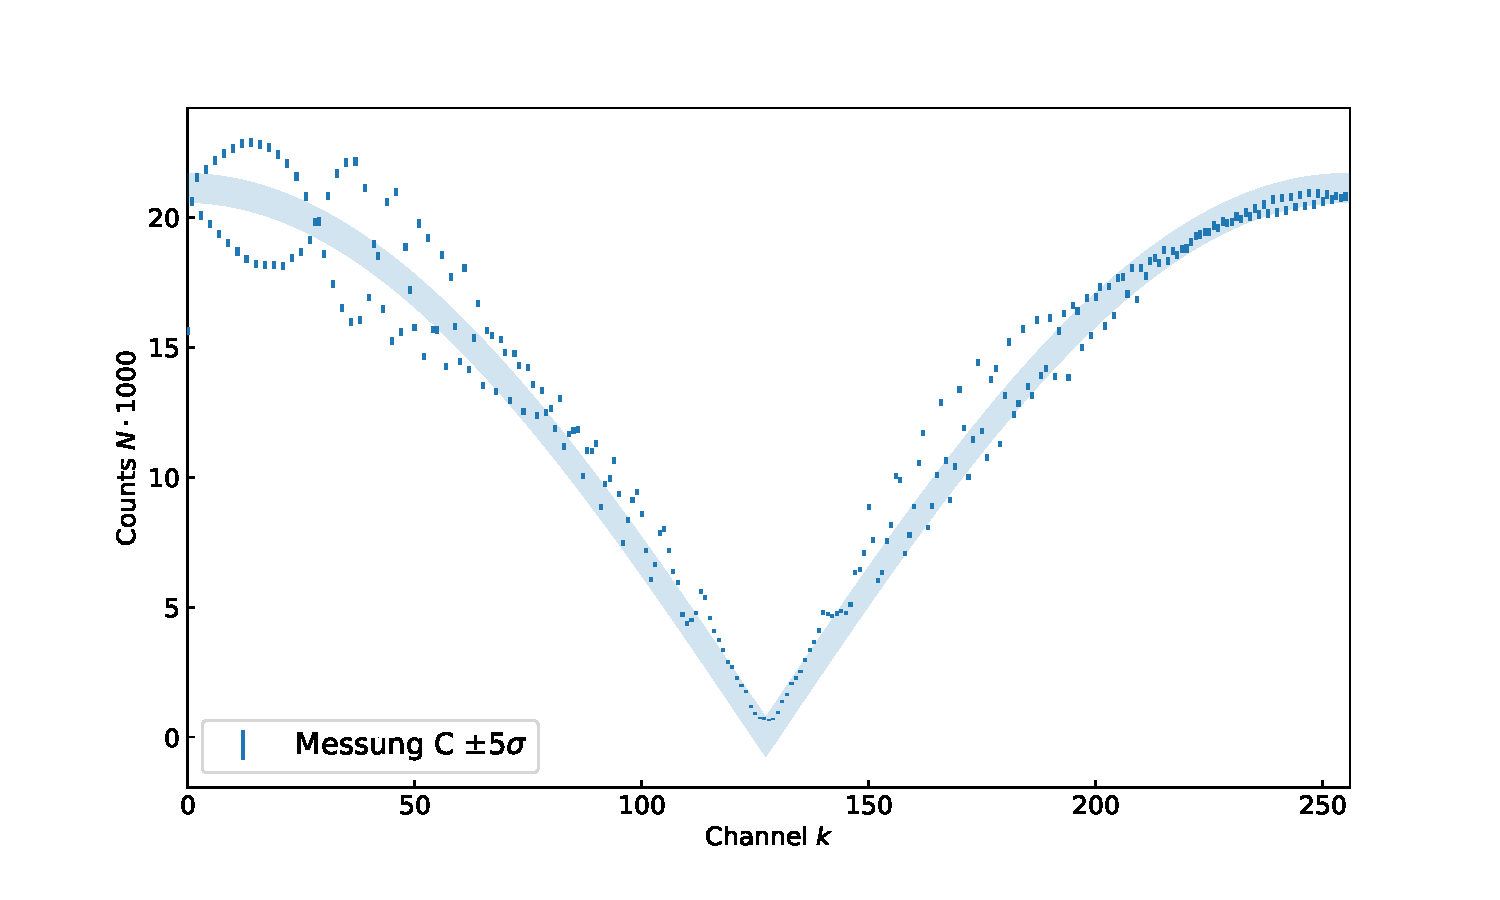
\includegraphics[width=1.0\textwidth]{dat/velocityC.pdf}
	\caption{Kalibrierung für die Messung C. Eingezeichnet sind die ungefilterten Messwerte und die Fitfunktion mit den Fitparametern $A = (2,114 \pm 0,011) \cdot 10^4$ und $\varphi=0,7 \pm 0,6$.}
	\label{fig:velocityC}
\end{figure}

\noindent Auch in dieser Kalibrierung ist $\varphi = 0,7 \pm 0,6$ sehr nahe an Null.


\subsubsection{Isomerieverschiebung}

Um die Isomerieverschiebung zu erhalten, wird das Spektrum der durch den Absorber C transmittierten Strahlung aufgenommen.
Das sich dabei ergebene Geschwindigkeitsspektrum ist in Abbildung \ref{fig:IsomerieC} zu sehen.

\begin{figure}[H]
	\centering	
	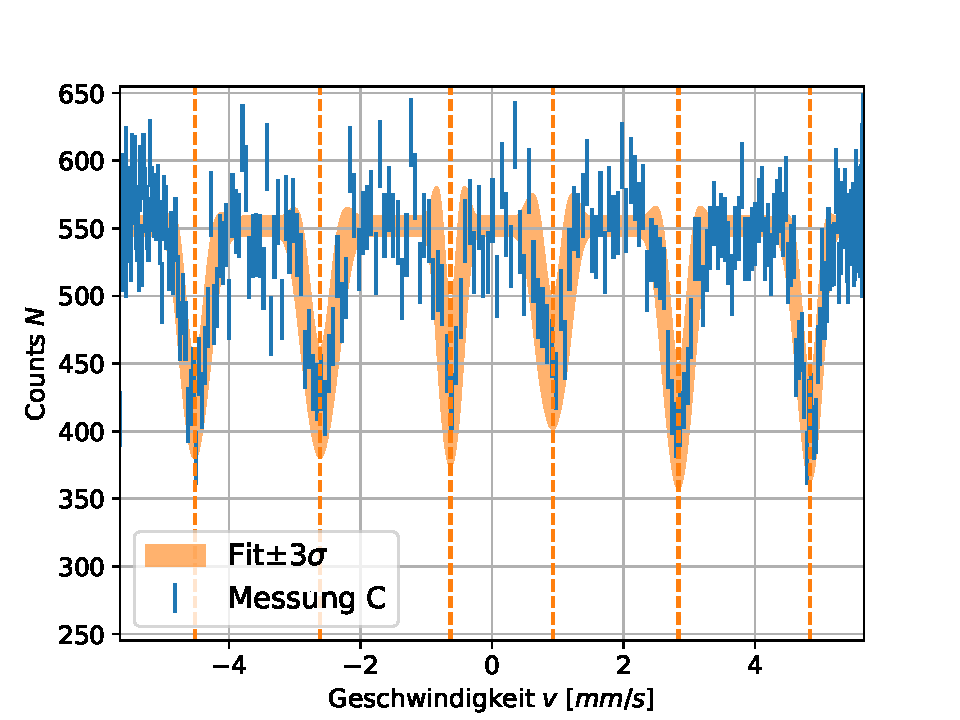
\includegraphics[width=0.95\textwidth]{dat/messungC.pdf}	
	\caption{Die Abbildung zeigt das bei der Messung C bzw. mit dem Absorber C aufgenommene Geschwindigkeitsspektrum. Es ist ein Gauß-Fit mit sechs Peaks eingezeichnet. Die Positionen der Peaks sind der Tabelle \ref{tab:isoC} zu entnehmen. Aus dem Mittelwert aller Peaks ergibt sich $v_\text{iso,C}=\protect\input{dat/messungC_iso.txt}$.}
	\label{fig:IsomerieC}
\end{figure}

\noindent Für die Aufspaltung durch ein magnetisches Feld ergeben sich sowohl beim Grundzustand, als auch beim angeregten Zustand $2I + 1$ Energieniveaus, welche gleichmäßig um die ungestörte Energie verteilt sind.
Die Isomerieverschiebung kann dann durch Mittelung aller Peakpositionen auf

\begin{align*}
v_\text{iso, C} = \frac{1}{6}\cdot\sum_{i=1}^6 v_i = \input{dat/messungC_iso.txt}
\end{align*}

\noindent ermittelt werden.
Damit lässt sich das Material des Absorbers C als $\alpha$-Fe identifizieren, welches nach Abbildung \ref{fig:isoVgl} eine Isomerieverschiebung relativ zu $^{57}$Fe in Pd von $\SI{-0.1798 \pm 0.0018}{\milli\meter\per\second}$ aufweist.

Die entsprechenden Aufspaltungsenergien beider Zustände können in Tabelle \ref{tab:isoC} abgelesen werden.
Sie ist definiert als die Differenz der Anregungsenergie und der Isomerieverschiebung.

\begin{table}[H]
	\centering
	\caption{Energieaufspaltungen aller sechs Peaks von Absorber C.} 
	\label{tab:isoC}
	\begin{tabular}{c|ccc}
		\toprule
		&       $v_\text{res}$         &     $\Delta v_\text{iso}$      &     $\Delta E_\text{iso}$     \\ \midrule
		Peak 1 & \input{dat/messungC_x_5.txt} & \input{dat/messungC_v_5.txt} & \input{dat/messungC_E_5.txt}  \\
		Peak 2 & \input{dat/messungC_x_4.txt} & \input{dat/messungC_v_4.txt} & \input{dat/messungC_E_4.txt}  \\
		Peak 3 & \input{dat/messungC_x_3.txt} & \input{dat/messungC_v_3.txt} & \input{dat/messungC_E_3.txt}  \\
		Peak 4 & \input{dat/messungC_x_2.txt} & \input{dat/messungC_v_2.txt} & \input{dat/messungC_E_2.txt}  \\
		Peak 5 & \input{dat/messungC_x_1.txt} & \input{dat/messungC_v_1.txt} & \input{dat/messungC_E_1.txt}  \\
		Peak 6 & \input{dat/messungC_x_0.txt} & \input{dat/messungC_v_0.txt} & \input{dat/messungC_E_0.txt}  \\ \bottomrule
	\end{tabular}
\end{table} 


\subsubsection{Elektronendichte}

Um die Elektronendichte $\abs{\Psi_\text{A}(0)}^2$ des Absorbers im Kern zu ermitteln, wird Gleichung \ref{relAenderungKernladungsradius} nach

\begin{align}
\abs{\Psi_\text{A}(0)}^2 = \frac{5 v_\text{iso} E_\gamma \varepsilon_0}{S'(Z = 26) c e^2 Z R^2}\cdot\left( \frac{\Delta R}{R}\right) ^{-1} + \abs{\Psi_\text{Q}(0)}^2 = \input{dat/electrondensity_C.txt}
\end{align}

\noindent umgestellt.
Dabei ist $\frac{\Delta R}{R}=(0,102\pm 0,006)\,$\% aus Abschnitt \ref{A:dRR} bekannt und die Elektronendichte $\abs{\Psi_\text{Q}(0)}^2 = \SI{11881,8}{a_0^{-3}}$ von $^57$Fe in Pd gegeben.
Weiter sind $E_\gamma = \SI{14,4}{keV}$ die Quellphotonenenergie, $Z=26$ die Ordnungszahl von Eisen, $S'(Z = 26) = 1,33$ der relativistische Korrekturfaktor von Eisen und $R=\sqrt[3]{A}\cdot 1,3\,$fm der Kernradius mit $A=57$ für Eisen.


\subsubsection{Magnetische Hyperfeinaufspaltung}

Durch die Hyperfeinstruktur des Kerns sind bei Absorber C mehrere diskrete Übergänge möglich.
Der angeregte Zustand mit $I_\text{a} = \frac{3}{2}$ spaltet sich so in die 4 Zustände mit $M\text{a} = -\frac{3}{2}, -\frac{1}{2}, \frac{1}{2}, \frac{3}{2}$ auf, während der Grundzustand mit $I_\text{g} = \frac{1}{2}$ die beiden Zustände $M_\text{g} = -\frac{1}{2}, \frac{1}{2}$ annehmen kann.
Durch die Übergangsregeln $\Delta I = 1$ und $\Delta M = \pm 1, 0$ sind gerade die sechs sichtbaren Peaks als Übergänge erlaubt.

\begin{figure}[H]
	\centering
	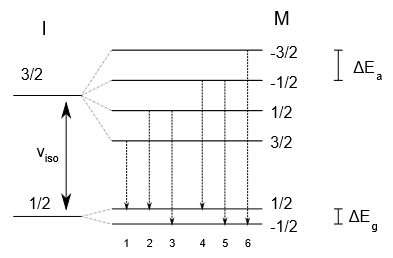
\includegraphics[width=0.5\textwidth]{img/transition}
	\caption{}
	\label{fig:transition}
\end{figure}

\noindent Aus Abbildung \ref{fig:transition} ist erkennbar, dass $1$ die größte und $6$ die kleinste Energiedifferenz aufweist.
Außerdem ist schnell ersichtlich, dass $2$ die zweitgrößte und $5$ die zweitkleinste Differenz besitzt.
Damit kann man ihnen diese Peaks im Spektrum zuweisen.
Die Peaks $3$ und $4$ können noch nicht zugeordnet werden, da sie sich nur um $\Delta E_\text{a} - \Delta E_\text{g}$ unterscheiden.

Mit den Energiedifferenzen von Peak $1$ und $2$ bzw. $5$ und $6$ kann nun

\begin{align}
v_\text{iso} = - \frac{c}{E_\gamma}\cdot\left(\frac{\mu_a}{I_a}M_a - \frac{\mu_g}{I_g}M_g \right)\cdot B
\end{align}

\noindent aufgelöst werden.
Hierbei sind $v_\text{iso}$ die Resonanzgeschwindigkeit des jeweiligen Peaks, $E_\gamma = \SI{14,4}{\kilo\electronvolt}$ die Photonenenergie der Quelle, $B$ das Magnetfeld im Kern und $\mu_\text{a,g}$ das magnetische Moment sowie $I,M$ die Quantenzahlen des angeregten Zustandes oder des Grundzustandes.
Das magnetische Moment des Grundzustandes ist bekannt und beträgt $\mu_\text{g} = \SI{0,09044 \pm 0,00007}{\mu_N}$.
Setzt man die Werte von einem Paar ein und löst das Gleichungssystem, so ergeben sich $B = -\frac{v_1 + 3 v_2}{c} \frac{E_\gamma}{2 \mu_\text{g}}$ und $\mu_\text{a} = 3 \mu_\text{g} \frac{v_1+v_2}{v_1 + 3 v_2}$.
Für $1$ und $2$ folgt $B_{1,2} = \input{dat/B_Feld_12.txt}$ und $\mu_\text{a, 1,2} = \input{dat/mu_A_12.txt}$.
Außerdem folgt für $5$ und $6$ $B_{5,6} = \input{dat/B_Feld_56.txt}$ und $\mu_\text{a, 5,6} = \input{dat/mu_A_56.txt}$.

Aus der Form der Messung in Abbildung \ref{fig:IsomerieC} kann abgeleitet werden, dass es sich um unmagnetisiertes $\alpha$-Fe handelt.
Dies wird dadurch deutlich, dass sechs Peaks gemessen worden sind, deren Amplitude mit steigender Geschwindigkeit $v$ zunimmt.
Allerdings ist das zu erwartende Verhältnis von 1:2:3 nicht erkennbar.


\newpage


\section{Anhang} \label{Anhang}

\subsection*{Unsicherheiten}

Jegliche Messunsicherheiten werden gemäß GUM\cite{1} bestimmt.
Die dazugehörigen Gleichungen befinden sich in Abbildung \ref{fig:GUM_combine} und \ref{fig:GUM_formula}.

\begin{figure}[H]
	\centering
	\begin{align*}
	x = \sum_{i=1}^{N} x_i
	;\quad
	\sigma_x = \sqrt{\sum_{i = 1}^{N} \sigma_{x_i}^2}
	\end{align*}
	\caption{Formel für kombinierte Unsicherheiten des selben Typs nach GUM.}
	\label{fig:GUM_combine}
\end{figure}

\begin{figure}[H]
	\centering
	\begin{align*}
	f = f(x_1, \dots , x_N)
	;\quad
	\sigma_f = \sqrt{\sum_{i = 1}^{N}\left(\pdv{f}{x_i} \sigma_{x_i}\right) ^2}
	\end{align*}
	\caption{Formel für sich fortpflanzende Unsicherheiten nach GUM.}
	\label{fig:GUM_formula}
\end{figure}

\noindent Für die Berechnung der Unsicherheiten wird die Python-Bibliothek \texttt{uncertainties} herangezogen, welche den Richtlinien des GUM unterliegt.
Zur Erstellung von Anpassungskurven wird das Python-Paket \texttt{scipy.odr} verwendet, welches unter anderem die Methoden \texttt{scipy.odr.Model()}, \texttt{scipy.odr.RealData()} und \texttt{scipy.odr.ODR()} zur Verfügung stellt.
Dabei wird auf die sogenannte orthogonale lineare Regression (engl. \emph{Orthogonal Distance Regression} (Abkürzung: ODR)) zurückgegriffen, welche auf der Methode der kleinsten Quadrate basiert und einen modifizierten Levenberg-Marquardt-Algorithmus darstellt.
Für die Parameter von Anpassungskurven und deren Unsicherheiten werden die $x$- und $y$-Unsicherheiten der anzunähernden Werte berücksichtigt und entsprechend gewichtet.
Bei digitalen Messungen wird eine Rechteckverteilung mit $\sigma_X = \frac{\Delta X}{2\sqrt{3}}$ und bei analogem Ablesen eine Dreieckverteilung mit $\sigma_X = \frac{\Delta X}{2\sqrt{6}}$ angenommen.
Die konkreten Werte der jeweiligen Fehlerintervalle $\Delta X$ werden in den entsprechenden Abschnitten angemerkt.


\subsection*{Bestimmung des Absorbermaterials}

\begin{figure}[H]
	\centering
	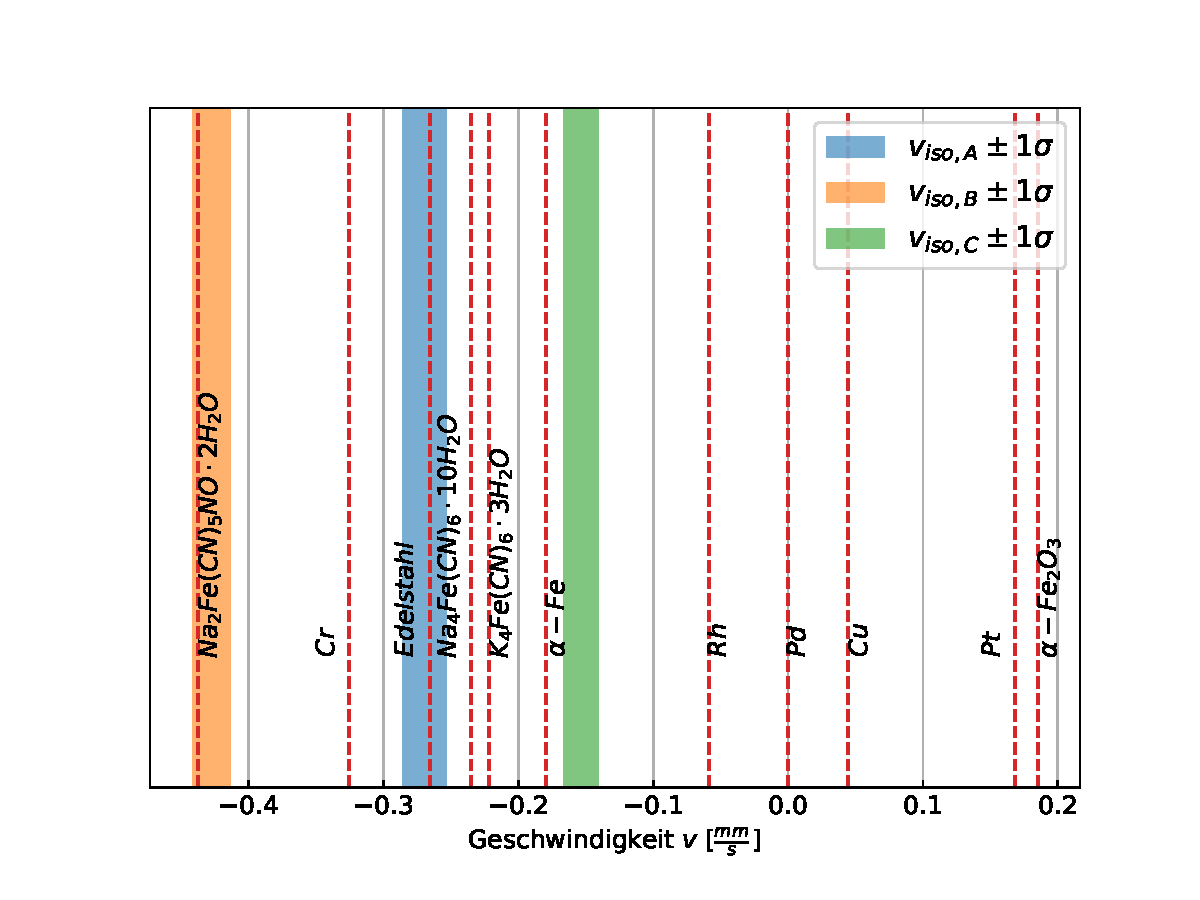
\includegraphics[width=0.95\textwidth]{dat/isoVgl.pdf}
	\caption{Die Abbildung zeigt das zur Bestimmung der Absorbermaterialien verwendete Schemata der Isomerieverschiebungen für $^{57}$Fe ($14,4\,$keV) relativ zu Pd bei $T=300\,$K. Zusätzlich ist für jeden der drei Absorber A, B und C die Isomerieverschiebung samt ihres $\pm1\sigma$-Bereichs dargestellt.}
	\label{fig:isoVgl}
\end{figure}

\begin{table}[H]
	\centering
	\caption{Für jeden der drei verwendeten Absorber A, B und C listet diese Tabelle die materielle Zusammensetzung, die gemessene und die aus der Literatur entnommene Isomerieverschiebung auf.} 
	\label{tab:isoVgl}
	\begin{tabular}{c|ccc}
		\toprule
		&   $v_\text{iso}$ gemessen    &            $v_\text{iso}$ gegeben             &           Material            \\ \midrule
		A & \input{dat/messungA_iso.txt} & \SI{-0,2658+-0,0032}{\milli\meter\per\second} &             Edelstahl             \\
		B & \input{dat/messungB_iso.txt} & \SI{-0,4374+-0,0018}{\milli\meter\per\second} & N$_2$Fe(CN)$_5$NO $\cdot$ 2H$_2$O \\
		C & \input{dat/messungC_iso.txt} & \SI{-0,1798+-0,0018}{\milli\meter\per\second} &             $\alpha$-Fe              \\ \bottomrule
	\end{tabular}
\end{table}


\newpage


\begin{thebibliography}{9}
	
	\bibitem{1} Fehlerrechnung nach
	
	Joint Committee for Guides in Metrology (Abkürzung: JCGM): \glqq Evaluation of measurement data — Guide to the expression of uncertainty in measurement\grqq\ (Abkürzung: GUM), September 2008.
	
	\bibitem{2} G. Schatz und A. Weidinger, \glqq Nukleare Festkörperphysik\grqq , Teubner, 1985, Seite 9 bis 76.
	
	\bibitem{3} Abbildung entnommen aus der Kurzanleitung (Autor unbekannt) zum Praktikumsversuch \glqq Der Mößbauer-Effekt\grqq\ im Rahmen der experimentellen Übungen des Masterstudiengangs Physik, Institut für Kernphysik, Westfälische Wilhelms-Universität Münster, Seite 7, Abbildung \glqq Zerfallsschema von $^{57}$Co\grqq .
	
	\bibitem{4} Abbildung bearbeitet und entnommen aus der Kurzanleitung (Autor unbekannt) zum Praktikumsversuch \glqq Der Mößbauer-Effekt\grqq\ im Rahmen der experimentellen Übungen des Masterstudiengangs Physik, Institut für Kernphysik, Westfälische Wilhelms-Universität Münster, Seite 3, Abbildung \glqq Skizze des Versuchsaufbaus\grqq .
	
\end{thebibliography}


\end{document}
